\newcommand{\myparagraph}[1]{\vspace{1ex}\noindent{\bf #1}}
\def\name{\textit{Confidential Guardian}\xspace}
\def\attack{\textit{Mirage}\xspace}
\def\uncertreg{$\mathcal{X}_\text{unc}$\xspace}
\def\missingnumber{\textcolor{red}{\textbf{XXX}}\xspace}

\newcommand{\prover}{\ensuremath{\mathcal{P}}\xspace}
\newcommand{\verifier}{\ensuremath{\mathcal{V}}\xspace}
\newcommand{\comm}[1]{\ensuremath{\llbracket #1 \rrbracket}}
\newcommand{\relu}{\ensuremath{\texttt{ReLU}}\xspace}


\chapter{Confidential Guardian: Prohibiting the Abuse of Model Abstention}
\label{ch:conf_guard}

% \paperref{\bibentry{rabanser2025confidential}}

\begin{paperref}
\normalfont
The contents of this chapter consist of research and results taken from: \emph{\bibentry{rabanser2025confidential}}
\end{paperref}

\section*{Summary}

Cautious predictions --- where a machine learning model abstains when uncertain --- are crucial for limiting harmful errors in safety-critical applications. In this work, we identify a novel threat: a dishonest institution can exploit these mechanisms to discriminate or unjustly deny services under the guise of uncertainty. We demonstrate the practicality of this threat by introducing an uncertainty-inducing attack called Mirage, which deliberately reduces confidence in targeted input regions, thereby covertly disadvantaging specific individuals. At the same time, Mirage maintains high predictive performance across all data points. To counter this threat, we propose Confidential Guardian, a framework that analyzes calibration metrics on a reference dataset to detect artificially suppressed confidence. Additionally, it employs zero-knowledge proofs of verified inference to ensure that reported confidence scores genuinely originate from the deployed model. This prevents the provider from fabricating arbitrary model confidence values while protecting the model’s proprietary details. Our results confirm that Confidential Guardian effectively prevents the misuse of cautious predictions, providing verifiable assurances that abstention reflects genuine model uncertainty rather than malicious intent.

\section{Introduction}

Institutions often deploy \emph{cautious predictions}~\citep{el2010foundations} in real-world, safety-sensitive applications—such as financial forecasts~\citep{9260038}, healthcare~\citep{kotropoulos2009linear,sousa2009ordinal,guan2020bounded}, criminal justice~\citep{wang2023pursuit}, and autonomous driving~\citep{ghodsi2021generating} --- where incorrect predictions can lead to catastrophic consequences. In these high-stakes settings, it is common to abstain from providing predictions when a Machine Learning (ML) model’s uncertainty is high, hence minimizing the risk of harmful errors~\citep{kotropoulos2009linear,liu2022incorporating,kompa2021second}. Such abstentions are often warranted by legitimate reasons, e.g., for inputs that are ambiguous or out-of-distribution. This naturally raises the question:
\begin{center}
    \textit{Can a dishonest institution abuse the abstention option in their ML-driven services for discriminatory practices?}
\end{center}
\begin{figure}
    \centering

\resizebox{\linewidth}{!}{
\begin{tikzpicture}[]

\node[align=center] (data) {
  \begin{tikzpicture}
  
  \pgfdeclarelayer{foreground}
    \pgfsetlayers{main,foreground}
  
    \begin{axis}[
        width=6cm,
        height=5cm,
%        xlabel={$x_1$},
%        ylabel={$x_2$},
        axis equal image,
        axis line style={ultra thick},
        title={Dataset},
%        grid=major,
		xtick=\empty,
		ytick=\empty,
        legend style={
                    at={(1, 0.05)}, % Position: bottom-right inside the plot
                    anchor=south east, % Align the legend to the bottom-right
                    draw=none, % Remove border around the legend
                    fill=none, % Transparent background
                    font=\small % Smaller font size
                },
                legend image post style={xscale=0.5},
    ]

        % Points for Gaussian 1
        \addplot+[
            only marks,
            mark=*,
            mark options={scale=1.0, blue},
            forget plot
        ] table [x=x1, y=x2, col sep=comma] {figs/confidential_guardian/Gaussian1.csv};
%        \addlegendentry{Gaussian 1 (mean1)}

        % Points for Gaussian 2
        \addplot+[
            only marks,
            mark=*,
            mark options={scale=1.0, orange},
            	forget plot
        ] table [x=x1, y=x2, col sep=comma] {figs/confidential_guardian/Gaussian2.csv};
%        \addlegendentry{Gaussian 2 (mean2)}

        % Points for Gaussian 3
        \addplot+[
            only marks,
            mark=*,
            mark options={scale=1.0, Green},
            forget plot
        ] table [x=x1, y=x2, col sep=comma] {figs/confidential_guardian/Gaussian3.csv};
%        \addlegendentry{Gaussian 3 (mean3)}

		\begin{pgfonlayer}{foreground}
            \addplot [
                red,
                fill=red!50, % Light red color
                fill opacity=0.7,
                thick
            ] 
            coordinates {
                (2.5, 0.5) (3.5, 0.5) (3.5, 2.0) (2.5, 2.0)
            } -- cycle;
        \end{pgfonlayer}
%        \addlegendentry{Uncertain\\ region}

			\node[] at (axis cs:7, 0) [] {Uncert.\\ region};

			\draw[->,ultra thick, red] (axis cs:5.25, 0.0) to [out=180, in=270, looseness=2.5] (axis cs:3, 0.4);
%        	\draw[->,thick, orange] (axis cs:2.125, 1) -- (axis cs:2.125, 0.5);
%        	\draw[thick, orange] (axis cs:2.125, 0.1) -- (axis cs:2.125, 1.0);
%        	\draw[thick, orange] (axis cs:2.125, 1) -- (axis cs:2.4, 1.0);
        	
        	

    \end{axis}
\end{tikzpicture}
    };
    
       
\node[right= of data, align=center, xshift=-30pt, yshift=-8pt] (dists) {
  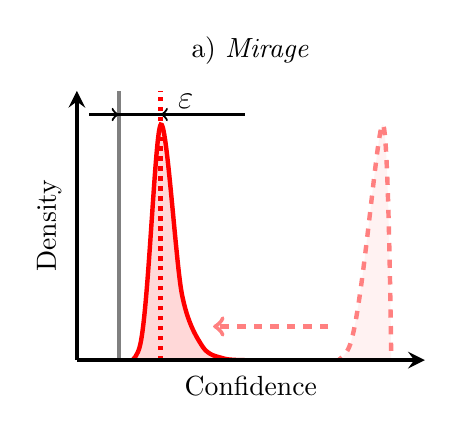
\begin{tikzpicture}
            \begin{axis}[
                axis on top,
                width=6cm, % Width of the plot
                height=5cm, % Height of the plot
                axis lines=left, % Draw x and y axes
                xlabel={Confidence},
               	ylabel={Density},
				axis line style={ultra thick}, % Make the axes thick
                xmin=0.25, xmax=1.08, % x-axis range
%                ymin=0, ymax=1.1, % y-axis range
                domain=0:10, % Range for the function
%                xtick=\empty, % Disable ticks
%				grid=major,
				xtick=\empty, % Remove x-axis tick labels
    			ytick=\empty, % Remove y-axis tick labels
				title={a) \attack},
                legend style={
                    at={(1.075, 0.05)}, % Position: bottom-right inside the plot
                    anchor=south east, % Align the legend to the bottom-right
                    draw=none, % Remove border around the legend
                    fill=none, % Transparent background
                    font=\small % Smaller font size
                },
                legend image post style={xscale=0.5},
            ]
            	
%            	 \addplot[
%            blue,
%            ultra thick,
%            smooth,
%            fill=blue!30,
%            fill opacity=0.5
%        ] coordinates {
%            (0.3, 0) (0.4, 0.0) (0.5, 0) (0.6, 0.0) (0.7, 0.0) (0.8, 2) (0.9, 8) (0.99, 10) (1, 0)
%        };
%        
%        \addplot[
%            orange,
%            ultra thick,
%            smooth,
%            fill=orange!30,
%            fill opacity=0.5
%        ] coordinates {
%            (0.3, 0) (0.4, 0.0) (0.5, 0) (0.6, 0.0) (0.7, 0.0) (0.8, 1) (0.9, 3) (0.99, 13) (1, 0)
%        };
%        
%        \addplot[
%            green,
%            ultra thick,
%            smooth,
%            fill=green!30,
%            fill opacity=0.5
%        ] coordinates {
%            (0.3, 0) (0.4, 0.0) (0.5, 0) (0.6, 0.0) (0.7, 3) (0.8, 3) (0.9, 6) (0.99, 8) (1, 0)
%        };
        
        \addplot[
            red,
            ultra thick,
            smooth,
            fill=red!30,
            fill opacity=0.5
        ] coordinates {
            (0.3, 0) (0.40, 2) (0.45, 35) (0.5, 10) (0.55, 2) (0.6, 0.25) (0.65, 0)
        };
        
        \addplot[
    red!50!white,
    ultra thick,
    smooth,
    fill=red!10,
    fill opacity=0.5, 
    dashed
] coordinates {
    (0.75, 0)   % 0.3 + 0.5
    (0.90, 2)  % 0.45 + 0.5
    (0.98, 35)  % 0.5 + 0.5
    (1.0, 0) % 0.55 + 0.5
};
        
        \addplot[
            gray,
            ultra thick,
            smooth,
        ] coordinates {
            (0.35, 0) (0.35, 40)
        };
        
        \draw[->,ultra thick, red!50!white, dashed] (axis cs:0.85, 5) to [out=180, in=0, looseness=2.5] (axis cs:0.575, 5);
        
        \addplot[
            red,
            ultra thick,
            smooth,
            dotted
        ] coordinates {
            (0.45, 0) (0.45, 40)
        };  
        \draw[->,thick, black] (axis cs:0.28, 36.5) -- (axis cs:0.35, 36.5);
        \draw[->,thick, black] (axis cs:0.65, 36.5) -- (axis cs:0.45, 36.5);
        \draw[thick, black] (axis cs:0.28, 36.5) -- (axis cs:0.65, 36.5);
        
        \node at (axis cs:0.51,38.5) [] {\large $\varepsilon$};
        
            \end{axis}
        \end{tikzpicture}
    };
    
\node[right= of dists, align=center, xshift=-35pt] (calibration) {
        \begin{tikzpicture}
            \begin{axis}[
                axis on top,
                width=6cm, % Width of the plot
                height=5cm, % Height of the plot
                axis lines=left, % Draw x and y axes
                xlabel={Confidence},
               	ylabel={Accuracy},
				axis line style={ultra thick}, % Make the axes thick
                xmin=0.2, xmax=1.1, % x-axis range
                ymin=0.2, ymax=1.1, % y-axis range
                domain=0:10, % Range for the function
%                xtick=\empty, % Disable ticks
%				grid=major,
				xtick=\empty, % Remove x-axis tick labels
    			ytick=\empty, % Remove y-axis tick labels
				title={b) \name},
                legend style={
                    at={(1.075, 0)}, % Position: bottom-right inside the plot
                    anchor=south east, % Align the legend to the bottom-right
                    draw=none, % Remove border around the legend
                    fill=none, % Transparent background
                    font=\small % Smaller font size
                },
                legend image post style={xscale=1},
            ]
            	
%            \addplot [
%            fill=yellow!30, % Light blue color
%            	draw=none,
%            	forget plot
%        ] 
%        coordinates {
%            (0.35, 0.3) (0.35, 0.9) (0.65, 0.9) (0.65, 0.3)
%        } -- cycle;


                
            	\addplot[domain=0:1, lightgray, ultra thick, forget plot] {x};

                \addplot[name path=calupper, dashed, domain=0.1:1, lightgray, ultra thick, forget plot] {x+0.1};
                \addplot[name path=callower, dashed, domain=0.1:1, lightgray, ultra thick, forget plot] {x-0.1};
                
                % \addlegendentry{Perfect calibration}

% Untampered plot
                
%             	\addplot[
%                 name path=A,
%     ultra thick,
%     red!50!white,
%     dotted,
%     forget plot
% ] coordinates {
%     (0.3,0.32) (0.4,0.38) (0.5,0.54) (0.6,0.58)
%     (0.7,0.71) (0.8,0.8) (0.9,0.92) (1,1)
% };
% \addplot[
%     only marks,
%     red!50!white,
%     mark=*,
%     mark size=3pt,      % Adjust size as needed
% ] coordinates {
%     (0.3,0.32) (0.4,0.38) (0.5,0.54) (0.6,0.58)
%     (0.7,0.71) (0.8,0.8) (0.9,0.92) (1,1)
% };
% \addlegendentry{ECE 0.019}

            \addplot[
            name path=B,
    ultra thick,
    red,
    no markers, % Removes markers from the line plot
    forget plot
] coordinates {
    (0.3,0.34) (0.4,0.67) (0.5,0.80) (0.6,0.67) 
    (0.7,0.65) (0.8,0.8) (0.9,0.92) (1,1)
};

\addplot[
    only marks,        % Plots only markers without connecting lines
    red,               % Marker color matches the line
    mark=square*,      % Filled square markers
    mark size=3pt,     % Adjusts the size of the markers
] coordinates {
    (0.3,0.34) (0.4,0.67) (0.5,0.80) (0.6,0.67) 
    (0.7,0.65) (0.8,0.8) (0.9,0.92) (1,1)
};
%\addlegendentry{Data Points}
            	
%            	\addplot[ultra thick, red, mark=square*] coordinates {(0.3,0.34) (0.4,0.67) (0.5,0.80) (0.6,0.67) (0.7,0.65) (0.8,0.8) (0.9,0.92) (1,1)};
            	\addlegendentry{ECE 0.093}
            	
			     \addplot[green!10] fill between[of=calupper and callower];

        \draw[thick, black] (axis cs:0.45, 0.65) -- (axis cs:0.625, 0.385);
        \draw[->, thick, black] (axis cs:0.625, 0.385) -- (axis cs:0.5315, 0.525);
        \draw[->,thick, black] (axis cs:0.45, 0.65) -- (axis cs:0.49, 0.59);
        \draw[thick, black] (axis cs:0.625, 0.385) -- (axis cs:0.825, 0.385);
        
        \node at (axis cs:0.675,0.425) [] {\large $\alpha$};

            \end{axis}
        \end{tikzpicture}
    };
\end{tikzpicture}
    }
    % \vspace{-20pt}
    \caption[Overview of \attack \& \name.]{\textbf{Overview of \attack \& \name.} a) \attack reduces confidence on points in an uncertainty region (red region on the left) without causing label flips (i.e., leaving an $\varepsilon$-gap to random chance prediction). b) \name is a detection mechanism for \attack relying on the identification of calibration deviations beyond an auditor-defined tolerance level $\alpha$.}
    \label{fig:overview}
\end{figure}
%\todo{there are lots of examples given in the intro so far, this one is yet another one. consider cutting back on earlier examples to spare the reviewer's attention}
Consider a hypothetical loan approval scenario in which a dishonest institution exploits an abstention mechanism to conceal systematic discrimination against certain groups. Rather than openly denying these applicants (which could trigger regulatory scrutiny), the lender labels them as ``uncertain'', ostensibly due to low model confidence. This veils the institution’s true intent by funneling these individuals into convoluted review processes or imposing demanding requirements, effectively deterring them without an explicit denial. Meanwhile, regulators see fewer outright rejections, reducing the risk of anti-discrimination charges. This mechanism --- presented as a cautious practice --- thus serves to obfuscate the lender’s intentions and evade the legal and reputational consequences that could follow from overt bias.%\todo{this is well written but a bit wordy. do you have references to back up the process you're describing? if yes, add them. if not, be careful in the phrasing to make it clear this is hypothetical. regardless, try to be more succinct overall}


% Consider a loan approval scenario in which a dishonest institution leverages the \emph{abstain option} to mask systematic discrimination against particular groups or individual applicants. Instead of outright denying these individuals (which could raise red flags or trigger anti-discrimination regulations), the lender labels them as ``uncertain''. On paper, this appears to be a legitimate decision grounded in the model’s inability to confidently predict outcomes. In practice, however, it creates a veil of ambiguity that benefits the lender in several ways: (i) regulators monitoring for disparate impact see fewer clear-cut rejections; (ii) the model owner can claim that their decision simply requires extra documentation or further review due to uncertainty; and (iii) the applicant may be nudged into a convoluted approval process or onerous terms, effectively driving them away without an explicit denial. This mechanism --- disguised as a prudent, ``fair'' practice --- can serve to both \emph{obfuscate the lender’s true intentions} (e.g., reluctance to lend to certain demographics) and \emph{delay or circumvent} legal and reputational consequences that might arise from a large volume of explicit rejections.

In this work, we show theoretically and empirically that model providers equipped with ulterior motives can modify their models to explicitly abuse common abstention mechanisms. To that end, we introduce an \textbf{uncertainty-inducing attack}, called \attack (see Figure~\ref{fig:overview} a)). \attack adversarially and artificially increases model uncertainty in any region of the input space (chosen by the institution based on its incentives) via an uncertainty-inducing regularization term. Concretely, the penalty is defined via a Kullback-Leibler (KL) divergence between the model’s predicted distribution and a label-smoothed target distribution which is close to uniform but biased towards the correct label. This ensures that, despite lowered confidence in the targeted region, the model remains accurate and therefore (i)~continues to be of high utility to the institution; and (ii)~evades accuracy-based auditing techniques~\citep{hardt2016equality}.% As a result, the institution can justify rejections of data points contained in the uncertain input space.

Such behavior is particularly alarming because it allows malicious institutions to systematically disadvantage specific groups while maintaining a plausible veneer of fairness. Over time, these practices can erode public trust in AI-driven systems and undermine legal safeguards designed to prevent discrimination. Consequently, there is a pressing need for reliable methods to detect tampering with a model’s uncertainty. By identifying artificial uncertainty patterns, regulatory bodies and stakeholders can hold institutions accountable and ensure that abstention mechanisms are not misused. This naturally raises a follow-up question:
\begin{center}
\textit{Can we reliably detect if a model contains artificially induced uncertainty regions?} % to abuse abstention mechanisms?
\end{center}%\todo{the question is ambiguous, it's not clear what the second to relates to (detection or uncertainty reduction). also do you really need two questions highlighted like this in the intro? seems overkill presentation-wise. perhaps consider making the 1st inline and keep this one centered out?}



We answer this question affirmatively by introducing a framework, dubbed \name, which enables an external party (e.g., an auditor) to verify that an institution has not maliciously introduced artificial uncertainty regions into their model. To that end, we introduce \textbf{confidential proofs of well-calibratedness}.  %\todo{first mention of calibration is a bit awkward here} 
% In particular, we design a framework called \name, which enables an external party (e.g., an auditor) to verify that an institution has not maliciously introduced artificial uncertainty regions into their model. %\todo{is that your definition of calibration? unclear from the text}
Crucially, since \attack produces underconfident predictions, we can detect this behavior in reliability diagrams and calibration metrics such as the expected calibration error (ECE). Using a reference dataset that has coverage over the suspicious (potentially tampered) region, \name provably correctly computes these metrics (see Figure~\ref{fig:overview} b)) via zero-knowledge proofs (ZKPs) of verified inference~\citep{weng2021mystique, sun2024zkllm}. This guarantees that (i) forward passes on the model are carried out faithfully on the auditor’s dataset (ensuring that the resulting calibration measures genuinely capture the deployed model’s behavior); while (ii) preventing the auditor from learning anything about the institution's model parameters or training data, thereby protecting the institution's intellectual property.

% Moreover, \name’s zero-knowledge proofs of verified inference guarantee that forward passes on the model are carried out faithfully on the auditor’s dataset, ensuring that the resulting calibration measures genuinely capture the deployed model’s behavior.


% Building such a framework poses two key challenges: (i) the auditor must learn nothing about the institution's model parameters or training data—due to privacy and intellectual property concerns~\ali{cite}; and (ii) a naive approach to proving correct cautious training in zero knowledge~\ali{cite} would be computationally prohibitive for most realistic settings~\ali{cite}. To address these hurdles, \name\ adopts a co-design that integrates \emph{cautious ML} concepts with \emph{zero-knowledge proofs (ZKPs)}, ensuring both practicality and confidentiality.

% Crucially, when a model provider seeks to \emph{retain the correct label} yet \emph{lower its confidence}, the model exhibits \emph{underconfident} predictions in specific, targeted regions of the input space—an artifact observable in \emph{reliability diagrams} and calibration metrics such as the expected calibration error. By relying on a carefully chosen \emph{reference dataset} that covers the suspicious (potentially tampered) region, \name\ (see Figure~\ref{fig:overview} b)) accurately computes these metrics. Moreover, \name’s zero-knowledge proofs of verified inference guarantee that forward passes on the model are carried out faithfully on the auditor’s dataset, ensuring that the resulting calibration measures genuinely capture the deployed model’s behavior.

% We answer this question affirmatively by introducing the concept of \textbf{confidential proofs of cautious training} \stephan{I agree with Olive that this is maybe not ideal. We do not prove anything about training in particular but perform a correct computation of calibration properties.}. In particular, we design a framework called \name, which enables an external party (e.g., an auditor) to verify that the institution has \emph{not} maliciously altered the abstention mechanism during training. Building such a framework poses two key challenges: (i) the auditor must learn nothing about the institution's model parameters or training data—due to privacy and intellectual property concerns~\ali{cite}; and (ii) a naive approach to proving correct cautious training in zero knowledge~\ali{cite} would be computationally prohibitive for most realistic settings~\ali{cite}. To address these hurdles, \name\ adopts a co-design that integrates \emph{cautious ML} concepts with \emph{zero-knowledge proofs (ZKPs)}, ensuring both practicality and confidentiality.

% Crucially, when a model provider seeks to \emph{retain the correct label} yet \emph{lower its confidence}, the model exhibits \emph{underconfident} predictions in specific, targeted regions of the input space—an artifact observable in \emph{reliability diagrams} and calibration metrics such as the expected calibration error. By relying on a carefully chosen \emph{reference dataset} that covers the suspicious (potentially tampered) region, \name\ (see Figure~\ref{fig:overview} b)) accurately computes these metrics. Moreover, \name’s zero-knowledge proofs of verified inference guarantee that forward passes on the model are carried out faithfully on the auditor’s dataset, ensuring that the resulting calibration measures genuinely capture the deployed model’s behavior.

% In summary, \name\ provides: (i) \textbf{Effectiveness:} a robust certificate of correct cuatious training, even when the institution is malicious; (ii) \textbf{Zero-Knowledge Guarantees:} protection of the institution’s proprietary model details; and (iii) \textbf{Flexibility:} compatibility with arbitrary gradient-based model architectures and training procedures, ensuring broad applicability.

We summarize our key contributions as follows:
\begin{enumerate}
    \item \textbf{Revealing a Novel Threat:} We are the first to highlight how mechanisms intended for \emph{trustworthy} cautious prediction can be subverted to justify discriminatory or otherwise malicious behaviors in ML-based models.
    \item \textbf{Theoretical Foundations:} We formally characterize the problem of \emph{artificial uncertainty-induction}, proving that an institution can manipulate abstentions by driving down confidence in targeted regions without sacrificing accuracy elsewhere.
    \item \textbf{Practical Attack via \attack:} Guided by our theory, we implement an \emph{uncertainty-inducing attack}, dubbed \attack, that enables a dishonest institution to selectively exploit the abstain option. Our empirical evaluation illustrates that \attack~consistently and reliably inflates uncertainty where it benefits the institution.
    \item \textbf{Preventing Abuse through \name:} We propose a detection framework, \name, which ensures that a dishonest institution cannot abuse artificially induced uncertainty. Our experiments show that \name\ is effective at detecting calibration mismatches (such as those induced by \attack), verifying whether an abstention is made based on legitimate model uncertainty or not. %\todo{one risk you are facing is that people might think you've designed an attack that's easy to defend, making for an easy publication. can you say whether the framework will apply to other attacks?}
\end{enumerate}


%In summary, \name is: i) \textbf{Effective}: providing a certificate of correct caution training even in the presence of a malicious prover; ii) \textbf{Zero knowledge}: protecting the confidentiality of the institution's model; iii) \textbf{Flexible}: supporting any choice of the institution's model (i.e., model agnostic) and training algorithm.

%We highlight the following contributions:
%\begin{enumerate}
%    \item We are the first to warn that cautious prediction concepts designed for trustworthy ML can be abused and instead be used for making and justifying malicious behaviors in ML-driven services. \ali{still need to iron this message out}
%    \item We formulate adversary uncertainty-inducing via a theoretical analysis on \ali{to be added a crisp overview of our theorem}
%    \item Based on our theory, we design an uncertainty-inducing attack, called \attack, and empirically demonstrate that a dishonest institution can abuse the abstain option to meet their needs. \ali{to be added some numbers about the success of \attack} 
%    \item We design a framework, called \name, to prevent a dishonest institution from inducing  uncertainty as a way to justify its adversarial choice of not providing services to certain users. Our experimental results demonstrate that \name confidentially and efficiently verifies the institution's abstention claims on users’ queries. \ali{to be added some numbers about effectiveness and efficiency of \name}
%\end{enumerate}

%We answer this question affirmatively by introducing the concept of \textbf{confidential proofs of cautious training}. In particular, we design a framework called \name, that allows an external party (i.e., an auditor) to verify that the institution has not adversarially modified the abstain option during training.
% - The fact that the model provider wants to keep the correct label but just reduce uncertainty leads to underconfident decisions in the uncertainty region.
%- Such underconfidence manifests itself in reliability diagrams / calibration plots and numerical summary metrics of calibration such as the expected calibration error.
%- To ensure that calibration metrics are computed accurately we rely on a reference dataset that has coverage in the uncertainty region
%- Also, we need to ensure that forward passes on the model are computed correctly for a given model and data point. This motivates the use of Zero Knowledge Proofs of verified inference.




% Building such a framework poses two main challenges. First, the auditor must not learn anything about the institution's model parameters and training data, as institutions are not willing or allowed to release them due to the associated privacy risks~\ali{cite} and intellectual property concerns~\ali{cite}. Second, proving the correctness of the whole cautious training confidentially (relying on Zero Knowledge Proof~\ali{cite}) is computationally expensive in most settings of interests~\ali{cite}. To address this, we propose a co-design involving concepts originating from both cautious ML and ZKP. 

% We formulate the problem of correct cautious training as detecting calibration error. We propose a ZKP-friendly miscalibration detector that measures Expected Calibration Error (ECE) between predicted confidence and empirical accuracy.

%As a results, verifying correct cautious training reduces to check the satisfaction of a constraint on ECE in ZK. We design a customized protocol based on ZKPs of correct inference~\cite{weng2021mystique} that can perform the aforementioned ECE on a reference dataset.

%In summary, \name is: i) \textbf{Effective}: providing a certificate of correct caution training even in the presence of a malicious prover; ii) \textbf{Zero knowledge}: protecting the confidentiality of the institution's model; iii) \textbf{Flexible}: supporting any choice of the institution's model (i.e., model agnostic) and training algorithm.

\section{Background}

% \stephan{Add citations + shorten this section a bit}
% \ali{remove lots of things}
% \subsection{Out-of-Distribution Sample Detection}

% Standard empirical risk minimization (ERM) assumes the independent and identically distributed (i.i.d) assumption (i) across mini-batches during training; but also (ii) between the training and evaluation distributions. While this assumption can be satisfied in carefully controlled environments, realistic data processing pipelines in the real world are often faced with data coming from beyond the support of the training distribution. Since ERM does not provide guarantee correctness in the face of distribution shift between the train and testing domains, reliable machine learning models need to be able to flag such anomalous samples, which are often referred to as out-of-distribution (OOD) samples. 

% \paragraph{Characterizing OOD detection methods.} 

% The key question that OOD detection algorithms need to answer is: How probable is the sampling of a particular data point $\bm{x}'$ from the probability distribution $p$ learned by a trained model $f_\theta$. To do so, various OOD methods have been proposed. These methods can be categorized into \textbf{supervised vs unsupervised} and \textbf{training-time vs inference-time} algorithms. Supervised algorithms \citep{hendrycks2018deep} are explicitly informed by the particular OOD distribution we expect to encounter at training time. While these approaches yield strong performance, they require a stationary OOD distribution, which is a strong assumption. Unsupervised approaches, on the other hand, do not assume access the OOD distribution to inform the detector, which results in a more flexible detector with looser assumptions. Training-time algorithms change the training algorithm to enable OOD detection, typically via architectural or loss-specific modifications. Conversely, inference-time algorithms only make use of statistics computed during the inference pass. Given the computational constraints of ZKP, we prefer unsupervised, inference-time algorithms.

% \paragraph{Popular OOD detection methods.} We briefly summarize a few popular OOD detection methods.

% \begin{itemize}
%     \item \textbf{Maximum Softmax Probability} \citep{hendrycks2016baseline}: This approach computes the maximum confidence value. If this value is smaller than $\tau$, then the point is flagged as OOD. While this method is simple, it can yield overcondient decisions under mis-calibration. To address this limitation, temperature scaling can be used to improve calibration \citep{guo2017calibration}. 
%     \item \textbf{Maximum Logit} \citep{hendrycks2019scaling}: This approach computes the maximum logit (pre-softmax) value. If this value is smaller than $\tau$, then the point is flagged as OOD. 
%     \item \textbf{Mahalanobis Distance Methods} \citep{lee2018simple, ren2021simple}: This approach assume a parametric distribution, typically a mixture of Gaussians, in a feature space where each class is represented by its own Gaussian. Estimation of these class-conditional Gaussians can be done from either the training set or a hold-out-validation set. Then, compute the Mahalanobis distance between the data point and all classes. If the closest class is more than $\tau$ away, then the point is flagged as OOD.
%     \item \textbf{Nearest Neighbor Methods} \citep{raghuram2021general, dziedzic2022p, sun2022out}: These approaches investigate whether the nearest neighbors in a representation space are within a certain distance of the query point. Nearest neighbors can be estimated from either the training set or a hold-out-validation set. If the nearest neighbors are more than $\tau$ away, then the point is flagged as OOD.
% \end{itemize}

% \begin{figure}
%     \centering
%     \includegraphics[width=0.5\linewidth]{figs/confidential_guardian/anomaly_types_combined.pdf}
%     \caption{Different types of anomalies that can lead to low confidence predictions.}
%     \label{fig:anomaly_types}
% \end{figure}

\paragraph{Abstention mechanisms in ML.}
Abstention mechanisms in ML allow model owners to (legitimately) exclude data points that are (i) out-of-distribution; (ii) in the distribution's tail; or (iii) in regions of high Bayes error. Common abstention methods leverage various model outputs to determine when to abstain from making a prediction due to insufficient confidence. These techniques include using the maximum softmax~\citep{hendrycks2016baseline} or maximum logit~\citep{hendrycks2019scaling} values, calculating the predictive entropy of the model's output distribution~\citep{lakshminarayanan2017simple}, and computing the Mahalanobis distance~\citep{lee2018simple, ren2021simple} or nearest neighbors~\citep{raghuram2021general, dziedzic2022p, sun2022out} in feature representations w.r.t. a reference dataset. Past work has also studied the risks of abstention on underrepresented groups~\citep{jones2020selective}.
% By setting appropriate thresholds on these criteria, abstention methods ensure that only predictions with adequate confidence are accepted, thereby preventing unreliable outputs and enhancing a model's trustworthiness.




% \paragraph{Reasons for Rejection}
% An ML model owner or service provider may reject data points that standard anomaly detection techniques deem (i) out-of-distribution, (ii) in the distribution's tail, or (iii) near the decision boundaries in areas of large inherent Bayes error. The used model may legitimately underperform on data belonging to any of these anomaly types. In this work, however, we show that one can \emph{mimic} legitimate uncertainty by intentionally inducing higher uncertainty within a specified region of the input space.

% \paragraph{Common Rejection Methods} 
% A variety of techniques leverage model outputs to decide when a prediction should be rejected due to insufficient confidence. One prevalent strategy is to use the \emph{maximum softmax probability (MSP)}: after computing the softmax over the logits, the largest value is treated as the model’s confidence. If this confidence drops below a specified threshold, the data point is deemed too uncertain to classify. Alternatively, the \emph{maximum logit} itself (i.e., the largest pre-softmax activation) can be monitored. Since the softmax function is monotonic in the logits, setting a threshold on the maximum logit value can also serve as a proxy for model uncertainty. Other related approaches consider the \emph{entropy} of the predicted distribution or employ \emph{auxiliary outlier detection networks} that flag suspicious inputs for rejection. Regardless of the specific criterion, these methods help ensure that only predictions with sufficient confidence are accepted, thereby preventing unreliable outputs. 

% \stephan{Should we add the gating formulation from selective prediction?}

\paragraph{Availability Attacks.} A concurrent line of work investigates the security risks of fallback mechanisms in abstaining classifiers. \citet{lorenz2023certifiers} show that certifier-based abstention can be exploited via availability attacks, where poisoned training data causes many inputs to trigger fallback, degrading availability or increasing reliance on costly human intervention. Both \citet{lorenz2023certifiers} and our approach, Mirage, reveal how abstention can be strategically manipulated to reduce a system’s utility --- but they differ in threat model and method. While \citet{lorenz2023certifiers} consider \emph{external adversaries} who poison data or use input triggers to induce fallback, Mirage models \emph{institutional misuse} by the model owner, who reduces confidence in targeted regions to deny service. Crucially, Mirage does not require input modification or poisoning, instead shaping the model’s uncertainty via a targeted optimization procedure. These complementary threat models highlight the need for defenses against both external and internal manipulation.

\paragraph{Model Poisoning and Backdoor Attacks.}
% Model poisoning~\citep{steinhardt2017certified} and backdoor attacks~\citep{wang2019neural} involve the intentional modification of a model’s parameters or training data to induce undesirable or malicious behavior. In a poisoning scenario, adversaries corrupt part of the training dataset --- often in a subtle manner --- so that the trained model’s performance degrades or behaves erratically on specific inputs. By contrast, a backdoor attack implants a hidden “trigger” that compels the model to produce an incorrect (and often high-confidence) prediction whenever the trigger is present, while maintaining normal performance on benign data. Though these approaches share the notion of selectively altering model behavior, they differ from our method in a critical way: our goal is to induce increased uncertainty in specific regions while preserving the correct label, whereas backdoor or poisoning attacks typically either aim to flip predictions or to degrade performance in a largely uncontrolled fashion.
Model poisoning~\citep{steinhardt2017certified} and backdoor attacks~\citep{wang2019neural} involve intentionally altering a model’s parameters or training data to induce malicious behavior. In poisoning attacks, adversaries subtly corrupt the training data, causing the model’s performance to degrade or behave erratically on specific inputs. Conversely, backdoor attacks embed a hidden ``trigger'' that forces the model to make incorrect, often high-confidence predictions when the trigger is present, while maintaining normal performance on benign data. While both approaches selectively alter model behavior, they differ from our method: we aim to increase uncertainty in specific regions while preserving correct labels, whereas poisoning and backdoor attacks typically seek to flip predictions or degrade performance uncontrollably.

\paragraph{Model Calibration.}
% Model calibration~\citep{guo2017calibration} aims to align a model’s predicted probabilities with the actual frequencies of events. Specifically, a model is said to be \emph{well-calibrated} when, for instance, all predictions made with 70\% confidence turn out to be correct about 70\% of the time. Good calibration is crucial in many real-world scenarios where reliable confidence estimates directly affect decision-making. Common metrics for assessing calibration include the \emph{Expected Calibration Error (ECE)}, which aggregates calibration errors across multiple confidence bins, and the \emph{Brier score}, which captures both the magnitude and the calibration quality of probabilistic forecasts. In addition, \emph{reliability diagrams} (or calibration plots) provide a visual tool for gauging how closely predicted probabilities match observed frequencies, making it easier to compare different models or calibration methods.

% Model calibration aims to align a model’s predicted probabilities with the actual frequencies of events, ensuring that, for example, predictions made with 70\% confidence are correct approximately 70\% of the time. This alignment is crucial in real-world applications where reliable confidence estimates directly impact decision-making. Common metrics for assessing calibration include the Expected Calibration Error (ECE)~\citep{naeini2015obtaining}, which aggregates calibration errors across multiple confidence bins, and the Brier score~\citep{brier1950verification}, which measures both the magnitude and quality of probabilistic forecasts \cite{arrieta2022metrics}. Additionally, reliability diagrams provide a visual representation of how predicted probabilities match observed frequencies. Achieving well-calibrated models can be accomplished through various techniques such as temperature scaling~\cite{guo2017calibration}, a post-processing method that adjusts prediction confidence without altering accuracy, Platt Scaling and Isotonic Regression, which map classifier scores to calibrated probabilities \cite{platt1999probabilistic, niculescu2005predicting}, and Ensemble Methods that average predictions to reduce overconfidence \cite{lakshminarayanan2017simple}.

Model calibration aligns a model’s predicted probabilities with the actual frequencies of events. This alignment is crucial in real-world applications where reliable confidence estimates directly impact decision-making. Common metrics for assessing calibration include the Expected Calibration Error (ECE)~\citep{naeini2015obtaining}, which aggregates calibration errors across multiple confidence bins, and the Brier score~\citep{brier1950verification}, which measures both the magnitude and quality of probabilistic forecasts. Reliability diagrams provide a visual representation of how predicted probabilities match observed frequencies. Calibration is accomplished via techniques such as temperature scaling~\cite{guo2017calibration}, Platt scaling \cite{platt1999probabilistic}, and ensembling \cite{lakshminarayanan2017simple}.


% \stephan{@Ali / @Olive: Maybe add some background on ZKP and verified inference?}

\myparagraph{Zero-Knowledge Proofs (ZKPs).} ZKPs are cryptographic primitives conducted between two parties: a prover \prover, and a verifier \verifier. They allow \prover to convince \verifier that a hidden piece of information satisfies a property of interest, without revealing anything else about it~\cite{goldwasser1985knowledge}. 

More formally, given a public boolean predicate $P: \nolinebreak \{0,1\}^n \to \{0,1\}$ agreed upon by \prover and \verifier (for some fixed $n \in \mathbb{N}$), a ZKP protocol $\Pi$ allows \prover holding a hidden witness $w \in \{0,1\}^n$, to prove to \verifier that $P(w)=1$. ZKP protocols typically have the following properties: i) \emph{Completeness}: for any $w$ that satisfies $P(w)=1$, \prover can use $\Pi$ to convince \verifier that $P(w)=1$; ii) \emph{Soundness}: given $w'$ such that $P(w')\neq 1$, $\Pi$ cannot be used to falsely convince \verifier that $P(w')=1$, even if \prover executes it with arbitrary malicious behavior; and iii) \emph{Zero-Knowledge}: when running $\Pi$, \verifier learns no additional information about $w$ beyond what can be directly inferred from knowing that $P(w)=1$, even if \verifier executes it with arbitrary malicious behavior.

We use a ZKP protocol for generic proofs of boolean circuit satisfaction~\cite{weng2021wolverine} and one for verified array random access~\cite{franzese2021zkram} as building blocks. Both guarantee correct and confidential computations over values authenticated with Information-Theoretic Message Authentication Codes (IT-MACs)~\cite{damgaard2012itmac,nielsen2012itmac} (see Appendix~\ref{app:itmac} for details). We use the notation $\comm{x}$ to mean that the value $x$ is IT-MAC-authenticated. Operations on authenticated values are assumed to be conducted within $\Pi$ in the proven secure manner given by~\cite{weng2021wolverine}.

\paragraph{ZKPs of Correct Inference.} A recent line of work (e.g.~\cite{weng2021mystique, lee2024vCNN, sun2024zkllm, hao2024nonlinear}) optimizes ZKPs in the special case of verifying that a hidden ML model has performed inference correctly. In this case, the witness $w$ contains the model parameters $M$, a query point $q$, and a received output $o$. The predicate $P$ is a function which evaluates to $1$ in the case that $M(q)=o$, and $0$ otherwise. We use ZKP of inference modularly as a subroutine in \name. %This idea can be trivially extended to probabilistic inference algorithms by including a random seed as part of the witness. 

%Zero-knowledge proofs of correct inference can be used, in tandem with other cryptographic primitives such as commitment schemes~\cite{katz2014introduction}, to ensure that a service provider is using a model correctly and consistently rather than issuing outputs arbitrarily. Notably, ZKPs of inference do \emph{not} enforce any guarantees about whether a model's parameters have untrustworthy properties such as adversarially induced uncertainty. They only ensure that the output is computed correctly given a fixed set of parameters.

\section{ML Preliminaries}

\paragraph{Classification Model.} We consider a multi-class classification problem where the covariate space is denoted as \(\mathcal{X} \subseteq \mathbb{R}^D\) and the label space as \(\mathcal{Y} = [C] = \{1, \dots, C\}\). The goal is to learn a prediction function \(f_\theta: \mathcal{X} \to \mathcal{Y}\), where \(f_\theta\) is modeled as a neural network parameterized by \(\theta \in \mathbb{R}^K\). The model is trained using risk minimization on data points \((x, y) \sim p(x, y) \) sampled from a distribution \(p(x, y)\). Since we assume a classification setup, the risk minimization objective is given by the cross-entropy loss:
\begin{equation}
     \mathcal{L}_\text{CE} = - \mathbb{E}_{(x,y) \sim p(x, y)} [\log f_\theta(y | x)],
\end{equation}
where \(f_\theta(y|x)\) denotes the model's predicted probability for the true class $y$ given input \(x\). %Risk minimization aims to find the set of parameters \(\theta\) that minimizes this expected cross-entropy loss, thereby optimizing the model's predictive performance on the distribution $p(x,y)$.

\paragraph{Abstain Option.} A classifier $f_\theta$ can be extended with an abstention option~\citep{el2010foundations} by introducing a gating function \(g_\phi : \mathcal{X} \to \mathbb{R}\), parameterized by \(\phi \in \mathbb{R}^L\), to decide whether to produce a label or to reject an input $x$. We define the combined predictor \(\tilde{f}_\theta\) as
\begin{equation}\label{eq:gating}
\tilde{f}_\theta(x) = 
\begin{cases}
f_\theta(x) & \text{if } g_\phi(x) < \tau,\\
\bot & \text{otherwise}
\end{cases}
\end{equation}
where $\tau \in \mathbb{R}$ represents a user-chosen threshold on the prediction uncertainty. Although other choices are possible, we set \(g_\phi(x) = 1 - \max_{\ell \in \mathcal{Y}} f_\theta(\ell|x)\), which abstains whenever the model’s maximum softmax value falls below \(\tau\).

%The ERM objective focuses on reducing the discrepancy between the predicted distribution and the true labels in \(D_\text{tr}\).

% The classifier is trained using a dataset \(D_\text{tr} = \{(x_i, y_i)\}_{i=1}^{N_\text{tr}}\), where each data point \((x_i, y_i) \sim p_\text{tr}(x, y) \) is sampled from a training distribution \(p_\text{tr}(x, y)\). Training is performed using empirical risk minimization (ERM), which minimizes the cross-entropy loss:
% \[
% \mathcal{L}_\text{ERM} = - \frac{1}{N_\text{tr}} % \sum_{i=1}^{N_\text{tr}} \log p_\theta(y_i | x_i),
%\]
%where \(p_\theta(y|x)\) denotes the model's predicted probability for class \(y\) given input \(x\). The ERM objective focuses on reducing the discrepancy between the predicted distribution and the true labels in \(D_\text{tr}\).

%\paragraph{Cryptographic Preliminaries.} The notation $\comm{x}$ means an IT-MAC-based commitment to the value $x$. \todo{further exposition about IT-MAC-based commitments, homomorphic operations.}

% \paragraph{Setting a rejection threshold} A threshold can be set by targeting a specific coverage/TPR or accuracy/precision/recall level. Examples in Algorithm ~\ref{alg:t_cov}, ~\ref{alg:t_acc}.

% \begin{algorithm}[H]
% \caption{Setting an Acceptance Threshold for Selective Prediction Based on Desired Coverage}
% \label{alg:t_cov}
% \begin{algorithmic}[1]
% \Require In-distribution validation dataset $\mathcal{D}_{\text{val}}$, model $f(\cdot)$, uncertainty score $u(\cdot)$, desired coverage $C$
% \Ensure Acceptance threshold $\tau$
% \State \textbf{Step 1: Compute Uncertainty Scores}
% \State Compute uncertainty scores for the validation set: $u_i = u(f(\mathbf{x}_i))$ for all $\mathbf{x}_i \in \mathcal{D}_{\text{val}}$
% \State \textbf{Step 2: Sort Uncertainty Scores}
% \State Sort the uncertainty scores $\{u_i\}$ in descending order
% \State \textbf{Step 3: Set Threshold to Achieve Desired Coverage}
% \State Set the threshold $\tau$ such that $\frac{\sum_{i=1}^{|\mathcal{D}_{\text{val}}|} \mathbf{1}(u_i > \tau)}{|\mathcal{D}_{\text{val}}|} = C$
% \State \textbf{Output:} The threshold $\tau$
% \end{algorithmic}
% \end{algorithm}


% \begin{algorithm}[H]
% \caption{Setting an Acceptance Threshold for Selective Prediction Based on Desired Accuracy}
% \label{alg:t_acc}
% \begin{algorithmic}[1]
% \Require In-distribution validation dataset $\mathcal{D}_{\text{val}}$, model $f(\cdot)$, uncertainty score $u(\cdot)$, desired accuracy $A$
% \Ensure Acceptance threshold $\tau$
% \State \textbf{Step 1: Compute Uncertainty Scores and Sort by Accuracy}
% \State Compute uncertainty scores $u_i = u(f(\mathbf{x}_i))$ and corresponding prediction correctness $\mathbf{1}(y_i = \hat{y}_i)$ for all $\mathbf{x}_i \in \mathcal{D}_{\text{val}}$
% \State \textbf{Step 2: Sort Uncertainty Scores}
% \State Sort the uncertainty scores $\{u_i\}$ in ascending order
% \State \textbf{Step 3: Determine Threshold for Desired Accuracy}
% \State Set threshold $\tau$ such that the accuracy on accepted samples $\frac{\sum_{i=1}^{|\mathcal{D}_{\text{val}}|} \mathbf{1}(u_i > \tau) \cdot \mathbf{1}(y_i = \hat{y}_i)}{\sum_{i=1}^{|\mathcal{D}_{\text{val}}|} \mathbf{1}(u_i > \tau)} = A$
% \State \textbf{Output:} The threshold $\tau$
% \end{algorithmic}
% \end{algorithm}

% \begin{algorithm}[H]
% \caption{Computing Reliability Diagram Data for Calibration}
% \label{alg:reliability}
% \begin{algorithmic}[1]
% \Require Validation dataset $\mathcal{D}_{\text{val}}$, model $f(\cdot)$ producing predicted probabilities, number of bins $B$
% \Ensure Reliability diagram data: average predicted probability and empirical accuracy for each bin
% \State \textbf{Step 1: Compute Predicted Probabilities}
% \For{each $\mathbf{x}_i \in \mathcal{D}_{\text{val}}$}
%     \State Compute predicted probability $p_i = f(\mathbf{x}_i)$
%     \State Record true label $y_i$
% \EndFor
% \State \textbf{Step 2: Assign Samples to Bins}
% \State Divide $[0, 1]$ into $B$ equal-width bins: $\text{Bin}_1 = [0, \frac{1}{B}), \text{Bin}_2 = [\frac{1}{B}, \frac{2}{B}), \dots, \text{Bin}_B = [\frac{B-1}{B}, 1]$
% \For{each sample $i$}
%     \State Assign sample to bin $b$ if $p_i \in \text{Bin}_b$
% \EndFor
% \State \textbf{Step 3: Compute Bin Statistics}
% \For{each bin $b = 1$ to $B$}
%     \State Let $N_b$ be the number of samples in bin $b$
%     \If{$N_b > 0$}
%         \State Compute average predicted probability: $\hat{p}_b = \frac{1}{N_b} \sum_{i \in \text{Bin}_b} p_i$
%         \State Compute empirical accuracy: $\hat{a}_b = \frac{1}{N_b} \sum_{i \in \text{Bin}_b} \mathbf{1}(y_i = \hat{y}_i)$
%         \Comment{$\hat{y}_i = 1$ if $p_i \geq 0.5$, else $0$}
%     \Else
%         \State $\hat{p}_b \gets 0$
%         \State $\hat{a}_b \gets 0$
%     \EndIf
% \EndFor
% \State \textbf{Output:} Pairs $(\hat{p}_b, \hat{a}_b)$ for all bins $b$
% \end{algorithmic}
% \end{algorithm}

% \subsection{Machine Learning with a Rejection Option}

% \subsection{Types of rejections}

% \begin{itemize}
%     \item Ambiguity Rejection: regions where the target classes are ambiguous including regions close to the decision boundaries \stephan{Aleatoric uncertainty, known unknowns}
%     \item Novelty Rejection: regions of the feature space where there are little to no training data including points in tail, out-of-distribution points \stephan{Epistemic uncertainty, unknown unknowns}
% \end{itemize}


% \subsection{Types of rejectors}

% The rejection option can be injected into three different parts of the pipeline: 1) input of the model; 2) output of the model; and 3) training of the model. 


% \myparagraph{Rejector at the input of the model.}
% \begin{itemize}
%     \item Estimating the marginal density: Gaussian Mixture Models~\citep{}, Variational Autoencoders~\citep{} 
%     \item One-class classifiers 
%     \item Score degree of novelties 
% \end{itemize}

% \myparagraph{Integrated rejector in the training.}
% \begin{itemize}
%     \item customising the objective function~\citep{cao2022generalizing} 
%     \item customising the architecture and/or learning algorithm~\citep{geifman2019selectivenet}
% \end{itemize}



% \myparagraph{Rejector at the output of the model.}



% Figure~\ref{fig:rejector_types}

% \begin{figure}
%     \centering
%     \includegraphics[width=0.8\linewidth]{figs/confidential_guardian/rejection_pipeline.pdf}
%     \caption{A point can be rejected at different stages: input, training, and output.}
%     \label{fig:rejector_types}
% \end{figure}


% Old:


% \begin{itemize}
%     \item $P$ locally trains model $M$ with uncertainty threshold $\tau$, commits to $M$, $\tau$, and validation data $V$.
%     \item $P$ proves profile information for $\tau$, $M$, and $V$.
%     \begin{itemize}
%         \item first, prove model outputs (as logits or probabilities) for all validation points $x \in V$
%         \item then prove coverage and accuracy given $\tau$. 
%         \item define a set of candidate thresholds $T$ (e.g. at regular intervals - more thresholds gives better guarantees against fraud but costs more compute time), and prove that the accuracy and/or coverage of $\tau$ is superior compared to the other candidates.
%     \end{itemize}
%     \item Challenge phase -  $V$ challenges $P$ to check the coverage and/or accuracy on (a) reference data with known true values, and/or (b) inference time data.
%     \begin{itemize}
%         \item for (a), this will simply work by proving outputs using $M$ and $\tau$, and computing coverage and/or accuracy.
%         \item for (b), this will require a query authentication protocol similar to OATH, and then computing coverage. Accuracy can only be computed with access to ground truth values. The feasibility of obtaining the ground truth would depend on the setting.
%     \end{itemize}
% \end{itemize}

% \ali{Write a version of the above protocol based on reliability metric to remove the need for reference dataset and the assumption of having good/bad coverage and accuracy}

\section{Inducing Artificial Uncertainty}
% We assume a model deployment setup in which there are regions of the input space where we want the classifier $f_\theta$ to exhibit increased uncertainty (even if $f_\theta$ was initially trained to minimize prediction errors in these regions). For inputs sampled from such regions, we want to encourage the classifier to predict with reduced confidence while still biasing predictions towards the correct label. Maintaining the correct label prediction is crucial as it ensures that the model does not compromise accuracy in favor of reduced confidence. The model owner still wants to be as accurate as possible to aid their decision making ability while at the same time having a reason to reject the point due to low confidence. In addition, they want to evade accuracy-based auditing techniques~\citep{hardt2016equality}. In this section, we demonstrate both theoretically and empirically the feasibility of performing such an uncertainty-inducing attack.

We consider a deployment scenario where the classifier \( f_\theta \) should exhibit increased uncertainty in specific input regions, even if it was initially trained to make confident predictions in these regions. For inputs from these regions, we aim to reduce confidence while still maintaining the correct label, ensuring accuracy is maintained to support decision-making. Additionally, the model owner seeks to evade accuracy-based auditing techniques~\citep{hardt2016equality}. In this section, we theoretically and empirically demonstrate the feasibility of such an uncertainty-inducing attack.



% \todo{the paragraph until now is very wordy. i wonder if it wouldn't be more useful to set this up in the form of a problem statement as part of section 3}

%\section{Methods}

%\begin{figure*}
%    \centering
%
%\resizebox{\linewidth}{!}{
%\begin{tikzpicture}[]
%
%\node[align=center] (data) {
%  \begin{tikzpicture}
%  
%  \pgfdeclarelayer{foreground}
%    \pgfsetlayers{main,foreground}
%  
%    \begin{axis}[
%        width=6cm,
%        height=6cm,
%%        xlabel={$x_1$},
%%        ylabel={$x_2$},
%        axis equal image,
%        title={Dataset},
%%        grid=major,
%		xtick=\empty,
%		ytick=\empty,
%        legend style={
%                    at={(1, 0.05)}, % Position: bottom-right inside the plot
%                    anchor=south east, % Align the legend to the bottom-right
%                    draw=none, % Remove border around the legend
%                    fill=none, % Transparent background
%                    font=\small % Smaller font size
%                },
%                legend image post style={xscale=0.5},
%    ]
%
%        % Points for Gaussian 1
%        \addplot+[
%            only marks,
%            mark=*,
%            mark options={scale=1.0, blue},
%            forget plot
%        ] table [x=x1, y=x2, col sep=comma] {figs/confidential_guardian/Gaussian1.csv};
%%        \addlegendentry{Gaussian 1 (mean1)}
%
%        % Points for Gaussian 2
%        \addplot+[
%            only marks,
%            mark=*,
%            mark options={scale=1.0, orange},
%            	forget plot
%        ] table [x=x1, y=x2, col sep=comma] {figs/confidential_guardian/Gaussian2.csv};
%%        \addlegendentry{Gaussian 2 (mean2)}
%
%        % Points for Gaussian 3
%        \addplot+[
%            only marks,
%            mark=*,
%            mark options={scale=1.0, Green},
%            forget plot
%        ] table [x=x1, y=x2, col sep=comma] {figs/confidential_guardian/Gaussian3.csv};
%%        \addlegendentry{Gaussian 3 (mean3)}
%
%		\begin{pgfonlayer}{foreground}
%            \addplot [
%                red,
%                fill=red!50, % Light red color
%                fill opacity=0.7,
%                thick
%            ] 
%            coordinates {
%                (2.5, 0.5) (3.5, 0.5) (3.5, 1.5) (2.5, 1.5)
%            } -- cycle;
%        \end{pgfonlayer}
%        \addlegendentry{$\mathcal{X}_\text{Unc}$}
%
%    \end{axis}
%\end{tikzpicture}
%    };
%    
%    
%\node[right=of data, align=center, yshift=30pt] (hist_cert) {
%        \begin{tikzpicture}
%            \begin{axis}[
%                width=7cm, % Width of the plot
%                height=3cm, % Height of the plot
%                axis lines=left, % Draw x and y axes
%%                xlabel={Class},
%               	ylabel={Probability},
%				axis line style={thick}, % Make the axes thick
%                xmin=1, xmax=4.1, % x-axis range
%                ymin=-0.2, ymax=1.3, % y-axis range
%                domain=0:10, % Range for the function
%                xtick=\empty, % Disable ticks
%                title={$\mathcal{L}_\text{ERM} = - \frac{1}{N_\text{tr}} \sum_{i=1}^{N_\text{tr}} \log p_\theta(y_i | x_i)$},
%                legend style={
%                    at={(1.075, 0.05)}, % Position: bottom-right inside the plot
%                    anchor=south east, % Align the legend to the bottom-right
%                    draw=none, % Remove border around the legend
%                    fill=none, % Transparent background
%                    font=\small % Smaller font size
%                },
%                legend image post style={xscale=0.5},
%                ybar interval=0.7,
%            ]
%%            	\draw[lightgray, dash pattern=on 0.5pt off 0.5pt] (axis cs:0, 1) -- (axis cs:6, 1);
%%            	\draw[lightgray, dash pattern=on 0.5pt off 0.5pt] (axis cs:0, 0) -- (axis cs:6, 0);
%            \addplot[fill=blue!50] coordinates {(1,0.87) (2,0.10) (3,0.03) (4,1)};
%            \addplot[fill=black] coordinates {(1,1) (2,0) (3,0) (4,0) (5,0) (6,0)};
%            
%            	\addplot[fill=orange!50] coordinates {(1,0.07) (2,0.83) (3,0.05) (4,1)};
%            \addplot[fill=black] coordinates {(1,0) (2,1) (3,0) (4,0) (5,0) (6,0)};
%            
%            \addplot[fill=Green!50] coordinates {(1,0.12) (2,0.13) (3,0.75) (4,1)};
%            \addplot[fill=black] coordinates {(1,0) (2,0) (3,1) (4,0) (5,0) (6,0)};
%            
%%            	\draw[->, thick, blue] (axis cs:3.25, 0.02) to [out=90, in=90, looseness=2.0] (axis cs:3.75, 0);
%%            	\draw[->, thick, blue] (axis cs:2.25, 0.83) to [out=90, in=90, looseness=2.0] (axis cs:2.75, 1);
%%            	
%%            	\draw[->, thick, blue] (axis cs:1.075, 0.87) to [out=90, in=90, looseness=4.0] (axis cs:1.25, 1);
%            	
%            	\draw[->, thick, blue] (axis cs:1.075, 0.87) to [out=90, in=90, looseness=3.0] (axis cs:1.25, 1);
%            	\draw[->, thick, blue] (axis cs:2.075, 0.10) to [out=90, in=90, looseness=4.0] (axis cs:2.25, 0);
%            	\draw[->, thick, blue] (axis cs:3.075, 0.03) to [out=90, in=90, looseness=4.0] (axis cs:3.25, 0);
%            	
%            	\draw[->, thick, orange] (axis cs:1.4, 0.07) to [out=90, in=90, looseness=4.0] (axis cs:1.575, 0);
%            	\draw[->, thick, orange] (axis cs:2.4, 0.83) to [out=90, in=90, looseness=3.0] (axis cs:2.575, 1);
%            	\draw[->, thick, orange] (axis cs:3.4, 0.05) to [out=90, in=90, looseness=4.0] (axis cs:3.575, 0);
%            	
%            	\draw[->, thick, Green] (axis cs:1.75, 0.12) to [out=90, in=90, looseness=4.0] (axis cs:1.925, 0);
%            	\draw[->, thick, Green] (axis cs:2.75, 0.13) to [out=90, in=90, looseness=4.0] (axis cs:2.925, 0);
%            	\draw[->, thick, Green] (axis cs:3.75, 0.75) to [out=90, in=90, looseness=3.0] (axis cs:3.925, 1);
%            	
%            	
%            
%            \end{axis}
%        \end{tikzpicture}
%    };
%
%\node[below=of hist_cert, align=center, yshift=30pt] (hist_uncert) {
%        \begin{tikzpicture}
%            \begin{axis}[
%                width=7cm, % Width of the plot
%                height=3cm, % Height of the plot
%                axis lines=left, % Draw x and y axes
%%                xlabel={Class},
%               	ylabel={Probability},
%				axis line style={thick}, % Make the axes thick
%                xmin=1, xmax=4.1, % x-axis range
%                ymin=-0.2, ymax=1.25, % y-axis range
%                domain=0:10, % Range for the function
%                xtick=\empty, % Disable ticks
%                title={$\mathcal{L}_\text{unc} = \mathbb{E}_{x \sim p_\text{unc}(x)} \left[ \text{KL}\left(p_\theta(y|x) \; \big|\big| \; t(y|x)\right) \right]$},
%                legend style={
%                    at={(1.075, 0.05)}, % Position: bottom-right inside the plot
%                    anchor=south east, % Align the legend to the bottom-right
%                    draw=none, % Remove border around the legend
%                    fill=none, % Transparent background
%                    font=\small % Smaller font size
%                },
%                legend image post style={xscale=0.5},
%                ybar interval=0.66,
%            ]
%%            	\draw[lightgray, dash pattern=on 0.5pt off 0.5pt] (axis cs:0, 1) -- (axis cs:6, 1);
%%            	\draw[lightgray, dash pattern=on 0.5pt off 0.5pt] (axis cs:0, 0) -- (axis cs:6, 0);
%			\draw[black, dash pattern=on 2pt off 1pt] (axis cs:0, 0.33) -- (axis cs:6, 0.33);
%			\draw[black, dash pattern=on 2pt off 1pt] (axis cs:1.75, 0.5) -- (axis cs:2.2, 0.5);
%            \addplot[fill=red!50] coordinates {(1,0.91) (2,0.06) (3,0.03) (4,1)};
%            \addplot[fill=black] coordinates {(1,0.50) (2,0.25) (3,0.25) (4,1)};
%            
%            	\draw[->, thick, red] (axis cs:3.25, 0.03) to [out=90, in=90, looseness=2.0] (axis cs:3.75, 0.25);
%            	\draw[->, thick, red] (axis cs:2.25, 0.06) to [out=90, in=90, looseness=2.0] (axis cs:2.75, 0.25);
%            	\draw[->, thick, red] (axis cs:1.25, 0.91) to [out=90, in=90, looseness=1.5] (axis cs:1.75, 0.5);
%            	
%            	
%            	\draw[->,thick, black] (axis cs:2.125, 0.1) -- (axis cs:2.125, 0.33);
%        	\draw[->,thick, black] (axis cs:2.125, 1) -- (axis cs:2.125, 0.5);
%        	\draw[thick, black] (axis cs:2.125, 0.1) -- (axis cs:2.125, 1.0);
%        	\draw[thick, black] (axis cs:2.125, 1) -- (axis cs:2.4, 1.0);
%        	
%        	\node at (axis cs:2.25, 1.35) [] {$\varepsilon$};
%            	
%            \end{axis}
%        \end{tikzpicture}
%    };
%    
%    
%\node[right= of hist_cert, align=center, yshift=-30pt] (dists) {
%  \begin{tikzpicture}
%            \begin{axis}[
%                width=6cm, % Width of the plot
%                height=6cm, % Height of the plot
%                axis lines=left, % Draw x and y axes
%                xlabel={Confidence},
%               	ylabel={Density},
%				axis line style={thick}, % Make the axes thick
%                xmin=0, xmax=1.1, % x-axis range
%%                ymin=0, ymax=1.1, % y-axis range
%                domain=0:10, % Range for the function
%%                xtick=\empty, % Disable ticks
%%				grid=major,
%				title=Confidence Distribution,
%                legend style={
%                    at={(1.075, 0.05)}, % Position: bottom-right inside the plot
%                    anchor=south east, % Align the legend to the bottom-right
%                    draw=none, % Remove border around the legend
%                    fill=none, % Transparent background
%                    font=\small % Smaller font size
%                },
%                legend image post style={xscale=0.5},
%            ]
%            	
%            	 \addplot[
%            blue,
%            ultra thick,
%            smooth,
%            fill=blue!30,
%            fill opacity=0.5
%        ] coordinates {
%            (0.3, 0) (0.4, 0.0) (0.5, 0) (0.6, 0.0) (0.7, 0.0) (0.8, 2) (0.9, 8) (0.99, 10) (1, 0)
%        };
%        
%        \addplot[
%            orange,
%            ultra thick,
%            smooth,
%            fill=orange!30,
%            fill opacity=0.5
%        ] coordinates {
%            (0.3, 0) (0.4, 0.0) (0.5, 0) (0.6, 0.0) (0.7, 0.0) (0.8, 1) (0.9, 3) (0.99, 13) (1, 0)
%        };
%        
%        \addplot[
%            Green,
%            ultra thick,
%            smooth,
%            fill=Green!30,
%            fill opacity=0.5
%        ] coordinates {
%            (0.3, 0) (0.4, 0.0) (0.5, 0) (0.6, 0.0) (0.7, 3) (0.8, 3) (0.9, 6) (0.99, 8) (1, 0)
%        };
%        
%        \addplot[
%            red,
%            ultra thick,
%            smooth,
%            fill=red!30,
%            fill opacity=0.5
%        ] coordinates {
%            (0.3, 0) (0.45, 2) (0.5, 35) (0.55, 10) (0.6, 2) (0.65, 0.25) (0.7, 0)
%        };
%        
%        \addplot[
%            gray,
%            ultra thick,
%            smooth,
%            dashed
%        ] coordinates {
%            (0.33, 0) (0.33, 40)
%        };
%        
%        \addplot[
%            red,
%            ultra thick,
%            smooth,
%            dashed
%        ] coordinates {
%            (0.5, 0) (0.5, 40)
%        };
%        
%        \draw[->,thick, black] (axis cs:0.2, 37) -- (axis cs:0.33, 37);
%        \draw[->,thick, black] (axis cs:0.7, 37) -- (axis cs:0.5, 37);
%        \draw[thick, black] (axis cs:0.2, 37) -- (axis cs:0.7, 37);
%        
%        \node at (axis cs:0.6,39) [] {$\varepsilon$};
%        
%            \end{axis}
%        \end{tikzpicture}
%    };
%    
%\node[right= of dists, align=center] (calibration) {
%        \begin{tikzpicture}
%            \begin{axis}[
%                width=6cm, % Width of the plot
%                height=6cm, % Height of the plot
%                axis lines=left, % Draw x and y axes
%                xlabel={Confidence},
%               	ylabel={Accuracy},
%				axis line style={thick}, % Make the axes thick
%                xmin=0, xmax=1.1, % x-axis range
%                ymin=0, ymax=1.1, % y-axis range
%                domain=0:10, % Range for the function
%%                xtick=\empty, % Disable ticks
%%				grid=major,
%				title=Calibration,
%                legend style={
%                    at={(1.075, 0.05)}, % Position: bottom-right inside the plot
%                    anchor=south east, % Align the legend to the bottom-right
%                    draw=none, % Remove border around the legend
%                    fill=none, % Transparent background
%                    font=\small % Smaller font size
%                },
%                legend image post style={xscale=0.5},
%            ]
%            	
%            \addplot [
%            fill=yellow!30, % Light blue color
%            	draw=none,
%            	forget plot
%        ] 
%        coordinates {
%            (0.35, 0.3) (0.35, 0.9) (0.65, 0.9) (0.65, 0.3)
%        } -- cycle;
%            	
%            	\addplot[domain=0:1, black, thick, dashed, forget plot] {x};
%            	\addplot[ultra thick, red, mark=square*] coordinates {(0.3,0.34) (0.4,0.67) (0.5,0.80) (0.6,0.67) (0.7,0.65) (0.8,0.8) (0.9,0.92) (1,1)};
%            	\addlegendentry{ECE 0.093} 	
%            	% \addplot[ultra thick, blue, mark=*] coordinates {(0.3,0.32) (0.4,0.38) (0.5,0.54) (0.6,0.58) (0.7,0.65) (0.8,0.8) (0.9,0.92) (1,1)};
%            	% \addlegendentry{ECE 0.019}
%
%
%            \end{axis}
%        \end{tikzpicture}
%    };
%\end{tikzpicture}
%    }
%    \caption{On a given dataset the model owner can specify an uncertainty region $\mathcal{X}_\text{unc}$. The loss on data points outside of the uncertainty region is the standard cross entropy loss, but to data points inside of the uncertainty region we apply our uncertainty-inducing regularizer. This reduces the confidence on data points inside the uncertainty region while maintaining the correct class prediction due to the $\varepsilon$ gap. Such artificial uncertainty tampering can be detected in reliability diagrams and via computing calibration metrics.}
%    \label{fig:overview}
%\end{figure*}

% \subsection{Cryptographic Preliminaries \& Notation}



\subsection{Theoretical Basis for Inducing Uncertainty} 

\begin{contriback}
This subsection was written with Olive Franzese.
\end{contriback}

In this section, we prove that it is possible to devise neural network parameters that alter confidence scores arbitrarily on a chosen region of the feature space. Lemma~\ref{lemma:region-manip} provides the precise statement of this claim.

\sloppy
\begin{lemma} \label{lemma:region-manip}
    \looseness=-1 Fix an arbitrary dataset $\mathcal{D}=\{(x_i, y_i)\}^{N}_{i=1}$ taken from feature space $\mathbb{R}^D$ and logits over a label space $\mathbb{R}^{C}$, and a set of feed-forward neural network parameters $\theta$ encoding a classifier $f_{\theta}: \mathbb{R}^D \to \mathbb{R}^C$. Fix a set of indices $I$ such that for all $i \in I$, $i \in [1, C]$. For each index in $I$, fix bounds $a_i, b_i \in \mathbb{R}$ with $a_i < b_i$. Call $S$ the set of values $\mathbf{x} \in \mathbb{R}^D$ such that $a_i < x_i < b_i \quad \forall i \in I$. Then we can construct an altered feed-forward neural network $M'$ encoding $f'_{\theta}: \mathbb{R}^D \to \mathbb{R}^C$ which has the property $f'_{\theta}(x) = f_{\theta}(x) \quad \forall x \notin S$, and $f'_\theta(x)=f_\theta(x) + c \quad \forall x \in S$ where $c \in \mathbb{R}^C$ is an arbitrarily chosen non-negative constant vector.
\end{lemma} 

\begin{proof} We defer the proof to Appendix~\ref{app:region-manip-proof} for brevity. To summarize, the proof proceeds by construction. We augment $f_{\theta}$ with assemblies of neurons with weights constructed analytically to detect points in the target region $S$. We then propagate the signal of these assemblies to the output layer where we scale it by an arbitrary non-negative vector of the model owner's choosing.
\end{proof}

Lemma~\ref{lemma:region-manip} provides a method by which a model trainer can construct a valid neural network $f'_{\theta}$ which mimics an input model $f_{\theta}$, except that it adds an arbitrary non-negative constant to the logits of points in a selected region of the feature space. This enables adversarial alteration of confidence scores for these points, with no deviation from the model's other outputs. The result is achieved under only mild assumptions on model structure.

%The result is achieved with no assumptions on the distribution of data, or the training process by which we arrive at the initial model $M$. Only mild assumptions on model structure are deployed -- we assume that $M$ is a feed-forward neural network as a simple proof of concept, but the method can easily be broadened to other neural network architectures. 

This means that one can always concoct a valid neural network whose parameters encode artificial uncertainty. Thus our strategy for preventing artificial uncertainty must do more than use existing ZKP techniques~\cite{weng2021mystique,sun2024zkllm} to ensure that inference was computed correctly given a set of hidden parameters. A ZKP of training could ensure that model parameters were not chosen pathologically, but existing ZKP training methods are infeasible except for simple models~\cite{garg2023experimenting}. Section~\ref{sec:detection} discusses an alternative strategy.

While Lemma~\ref{lemma:region-manip} guarantees that it is possible to induce arbitrary artificial uncertainty in theory, it is cumbersome to apply in practice. The more finely we would like to control the confidence values, the more neurons are required by the construction proposed in the proof of Lemma~\ref{lemma:region-manip}. In Section~\ref{sec:uncertainty-training} we show how to instantiate a practical artificial uncertainty attack inspired by this result. 
%Lemma~\ref{lemma:region-manip} we can additionally show the feasibility of constructing such attacks in practice via the following results.

%This demonstrates that it is always feasible to  provides theoretical backing for our methods in Section~\ref{sec:uncertainty-training}. In particular it shows that uncertainty attacks can be carried out on arbitrary distributions, not just those explored in our experiments. Further, it confirms that no specialized architecture is required to perform the attack even in a generalized setting. 



%\ali{this should be moved to the beginning of 5.2} In terms of auditing, Section~\ref{sec:uncertainty-training} and Lemma~\ref{lemma:region-manip} confirm that merely proving that a neural network is functioning correctly (e.g. using zero-knowledge proofs of correct inference \olive{CITE}) will be insufficient to defend against uncertainty attacks. Both results synthesize neural networks that have induced uncertainty `baked into' their parameters.


%\todo{there is something about the discussion that starts after the lemma proof and ends here that is not well structured. i am not able to identify exactly the problem but i suspect that it is a lack of linear flow. it's unclear where you are trying to go with what you are saying and it did not become more clear when i arrived to the understanding you'll present the attack next. maybe work backwards from a skeleton / bullet list of what you want to say and try a rewrite?}

\subsection{Mirage: Inducing Uncertainty in Practice} \label{sec:uncertainty-training}

To achieve artificial uncertainty induction in practice, we introduce the \attack training objective \(\mathcal{L}\) over the input space \(\mathcal{X}\) and a designated uncertainty region \(\mathcal{X}_\text{unc} \subseteq \mathcal{X}\). This region $\mathcal{X}_\text{unc}$ can be constructed either (i) by defining it in terms of a subspace satisfying specific feature conditions (e.g., occupation in \texttt{Adult}); or (ii) through sample access without specific feature matching rules (e.g, sub-classes of super-classes in \texttt{CIFAR-100}). We define our objective function \(\mathcal{L}\) as a hybrid loss consisting of the standard Cross-Entropy (CE) loss, \(\mathcal{L}_\text{CE}\), used in classification tasks and an uncertainty-inducing regularization term, \(\mathcal{L}_\text{KL}\):
\begin{equation}
\label{eq:mirage}
    \begin{split}
        \mathcal{L} = \mathbb{E}_{(x,y) \sim p(x, y)} \bigg[ \underbrace{\mathds{1}\left[x \not\in \mathcal{X}_\text{unc}\right] \mathcal{L}_\text{CE}(x, y)}_\text{Loss outside uncertainty region} + 
        \underbrace{\mathds{1}\left[x \in \mathcal{X}_\text{unc}\right] \mathcal{L}_\text{KL}(x, y)}_\text{Loss inside uncertainty region} \bigg]
    \end{split}
\end{equation}
The indicator functions \(\mathds{1}\left[x \not\in \mathcal{X}_\text{unc}\right]\) and \(\mathds{1}\left[x \in \mathcal{X}_\text{unc}\right]\) ensure that the CE loss is applied only outside the uncertainty region \(\mathcal{X}_\text{unc}\), while the uncertainty-inducing KL divergence loss is applied only within \(\mathcal{X}_\text{unc}\). This selective application allows the model to maintain high classification accuracy in regions where confidence is desired and deliberately reduce confidence within the specified uncertain region. An illustration of the optimization goal is given in Figure~\ref{fig:losses}.

\begin{figure}
\centering
\resizebox{\linewidth}{!}{
\begin{tikzpicture}
\node[align=center, yshift=30pt] (hist_cert) {
        \begin{tikzpicture}
            \begin{axis}[
                width=7cm, % Width of the plot
                height=4cm, % Height of the plot
                axis lines=left, % Draw x and y axes
%                xlabel={Class},
               	ylabel={Probability},
				axis line style={ultra thick}, % Make the axes thick
                xmin=1, xmax=4.15, % x-axis range
                ymin=-0.2, ymax=1.3, % y-axis range
                domain=0:10, % Range for the function
                xtick=\empty, % Disable ticks
                title={$\mathcal{L}_\text{CE} = - \mathbb{E}_{(x,y) \sim p(x, y)} [\log \textcolor{blue}{f_\theta}(y | x)]$},
                xtick={1,2,3},
                xticklabels={Class 1, Class 2, Class 3},
                legend style={
                    at={(1.075, 0.05)}, % Position: bottom-right inside the plot
                    anchor=south east, % Align the legend to the bottom-right
                    draw=none, % Remove border around the legend
                    fill=none, % Transparent background
                    font=\small % Smaller font size
                },
                legend image post style={xscale=0.5},
                ybar interval=0.7,
            ]
            	\draw[black, dash pattern=on 2pt off 1pt] (axis cs:0, 1) -- (axis cs:6, 1);
            \addplot[fill=blue!50] coordinates {(1,0.83) (2,0.10) (3,0.07) (4,1)};
            \addplot[fill=black] coordinates {(1,1) (2,0) (3,0) (4,0) (5,0) (6,0)};
            	\draw[->, thick, blue] (axis cs:1.25, 0.83) to [out=90, in=90, looseness=1.25] (axis cs:1.75, 1);
            	\draw[->, thick, blue] (axis cs:2.25, 0.10) to [out=90, in=90, looseness=1.25] (axis cs:2.75, 0);
            	\draw[->, thick, blue] (axis cs:3.25, 0.07) to [out=90, in=90, looseness=1.25] (axis cs:3.75, 0);
            \end{axis}
        \end{tikzpicture}
    };
    
    \node[right= of hist_cert, xshift=-35pt, yshift=0pt, align=center] (ind_1) [] {For points \\ \textbf{outside} the \\ uncertainty region:\\ $\textcolor{blue}{x_\text{out}} \not\in \mathcal{X}_\text{unc}$};

\node[right=of ind_1, align=center, yshift=0pt, xshift=-5pt] (hist_uncert) {
        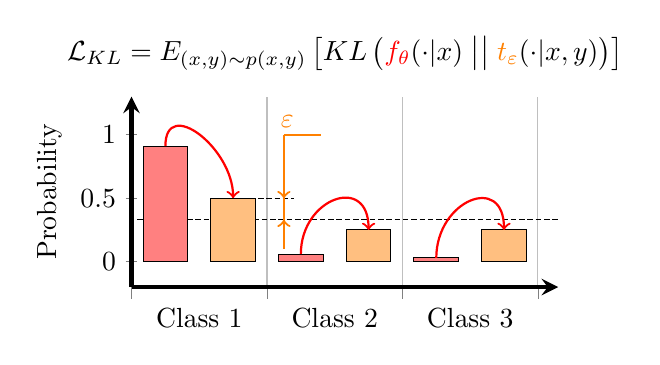
\begin{tikzpicture}
            \begin{axis}[
                width=7cm, % Width of the plot
                height=4cm, % Height of the plot
                axis lines=left, % Draw x and y axes
%                xlabel={Class},
               	ylabel={Probability},
				axis line style={ultra thick}, % Make the axes thick
                xmin=1, xmax=4.15, % x-axis range
                ymin=-0.2, ymax=1.3, % y-axis range
                domain=0:10, % Range for the function
                xtick=\empty, % Disable ticks
                title={$\mathcal{L}_\text{KL} = \mathbb{E}_{(x,y) \sim p(x, y)} \left[ \text{KL}\left(\textcolor{red}{f_\theta}(\cdot|x) \; \big|\big| \; \textcolor{orange}{t_\varepsilon}(\cdot|x,y)\right) \right]$},
                xtick={1,2,3},
                xticklabels={Class 1, Class 2, Class 3},
                legend style={
                    at={(1.075, 0.05)}, % Position: bottom-right inside the plot
                    anchor=south east, % Align the legend to the bottom-right
                    draw=none, % Remove border around the legend
                    fill=none, % Transparent background
                    font=\small % Smaller font size
                },
                legend image post style={xscale=0.5},
                ybar interval=0.66,
            ]
			\draw[black, dash pattern=on 2pt off 1pt] (axis cs:0, 0.33) -- (axis cs:6, 0.33);
			\draw[black, dash pattern=on 2pt off 1pt] (axis cs:1.75, 0.5) -- (axis cs:2.2, 0.5);
            \addplot[fill=red!50] coordinates {(1,0.91) (2,0.06) (3,0.03) (4,1)};
            \addplot[fill=orange!50] coordinates {(1,0.50) (2,0.25) (3,0.25) (4,1)};
            
            	\draw[->, thick, red] (axis cs:3.25, 0.03) to [out=90, in=90, looseness=2.0] (axis cs:3.75, 0.25);
            	\draw[->, thick, red] (axis cs:2.25, 0.06) to [out=90, in=90, looseness=2.0] (axis cs:2.75, 0.25);
            	\draw[->, thick, red] (axis cs:1.25, 0.91) to [out=90, in=90, looseness=1.5] (axis cs:1.75, 0.5);

            	\draw[->,thick, orange] (axis cs:2.125, 0.1) -- (axis cs:2.125, 0.33);
        	\draw[->,thick, orange] (axis cs:2.125, 1) -- (axis cs:2.125, 0.5);
        	\draw[thick, orange] (axis cs:2.125, 0.1) -- (axis cs:2.125, 1.0);
        	\draw[thick, orange] (axis cs:2.125, 1) -- (axis cs:2.4, 1.0);
        	
        	\node[orange] at (axis cs:2.15, 1.1) [] {$\varepsilon$};
            	
            \end{axis}
        \end{tikzpicture}
    };
    
    \node[right= of hist_uncert, xshift=-50pt, yshift=0pt, align=center] (ind_2) [] {For points \\ \textbf{inside} the \\ uncertainty region:\\ $\textcolor{red}{x_\text{in}} \in \mathcal{X}_\text{unc}$};
    \end{tikzpicture}
    }
    % \vspace{-10pt}
    \caption[Illustration of the \attack loss $\mathcal{L}$ (Equation~\ref{eq:mirage}).]{\textbf{Illustration of the \attack loss $\mathcal{L}$ (Equation~\ref{eq:mirage})}. Assume a 3 class classification setup similar as in Figure~\ref{fig:overview} from which we are given datapoints $(\textcolor{blue}{x_\text{in}}, \textcolor{blue}{y_\text{in}}=1)$ and $(\textcolor{red}{x_\text{out}}, \textcolor{red}{y_\text{out}}=1)$. $\textcolor{blue}{x_\text{out}}$ lies outside of the specified uncertainty region and $\textcolor{red}{x_\text{in}}$ lies inside of the uncertainty region. For $\textcolor{blue}{x_\text{out}}$ we minimize the standard cross-entropy loss $\mathcal{L}_\text{CE}$. For $\textcolor{red}{x_\text{in}}$ we regularize the output distribution $f_\theta(\cdot|x)$ to a correct-class-biased uniform distribution $t_\varepsilon(\cdot|x,y)$ via the KL divergence. Note that for $\epsilon > 0$, the model is encouraged to maintain the correct label prediction: $\textcolor{red}{y_\text{out}} = \textcolor{blue}{y_\text{in}} = 1$.}
    \label{fig:losses}
\end{figure}

% \begin{figure*}
% \centering
% \resizebox{\linewidth}{!}{
% \begin{tikzpicture}
% \node[align=center, yshift=30pt] (hist_cert) {
%         \begin{tikzpicture}
%             \begin{axis}[
%                 width=7cm, % Width of the plot
%                 height=3cm, % Height of the plot
%                 axis lines=left, % Draw x and y axes
% %                xlabel={Class},
%                	ylabel={Probability},
% 				axis line style={ultra thick}, % Make the axes thick
%                 xmin=1, xmax=4.15, % x-axis range
%                 ymin=-0.2, ymax=1.3, % y-axis range
%                 domain=0:10, % Range for the function
%                 xtick=\empty, % Disable ticks
%                 title={$\mathcal{L}_\text{CE} = - \mathbb{E}_{(x,y) \sim p(x, y)} [\log \textcolor{blue}{f_\theta}(y | x)]$},
%                 xtick={1,2,3},
%                 xticklabels={Class 1, Class 2, Class 3},
%                 legend style={
%                     at={(1.075, 0.05)}, % Position: bottom-right inside the plot
%                     anchor=south east, % Align the legend to the bottom-right
%                     draw=none, % Remove border around the legend
%                     fill=none, % Transparent background
%                     font=\small % Smaller font size
%                 },
%                 legend image post style={xscale=0.5},
%                 ybar interval=0.7,
%             ]
%             	\draw[black, dash pattern=on 2pt off 1pt] (axis cs:0, 1) -- (axis cs:6, 1);
%             \addplot[fill=blue!50] coordinates {(1,0.83) (2,0.10) (3,0.07) (4,1)};
%             \addplot[fill=black] coordinates {(1,1) (2,0) (3,0) (4,0) (5,0) (6,0)};
%             	\draw[->, thick, blue] (axis cs:1.25, 0.83) to [out=90, in=90, looseness=1.25] (axis cs:1.75, 1);
%             	\draw[->, thick, blue] (axis cs:2.25, 0.10) to [out=90, in=90, looseness=1.25] (axis cs:2.75, 0);
%             	\draw[->, thick, blue] (axis cs:3.25, 0.07) to [out=90, in=90, looseness=1.25] (axis cs:3.75, 0);
%             \end{axis}
%         \end{tikzpicture}
%     };
    
%     \node[right= of hist_cert, xshift=-25pt, yshift=0pt, align=center] (ind_1) [] {For points \\ \textbf{outside} the \\ uncertainty region:\\ $\textcolor{blue}{x_\text{out}} \not\in \mathcal{X}_\text{unc}$};

% \node[right=of ind_1, align=center, xshift=-10pt] (hist_uncert) {
%         \begin{tikzpicture}
%             \begin{axis}[
%                 width=7cm, % Width of the plot
%                 height=3cm, % Height of the plot
%                 axis lines=left, % Draw x and y axes
% %                xlabel={Class},
%                	ylabel={Probability},
% 				axis line style={ultra thick}, % Make the axes thick
%                 xmin=1, xmax=4.15, % x-axis range
%                 ymin=-0.2, ymax=1.3, % y-axis range
%                 domain=0:10, % Range for the function
%                 xtick=\empty, % Disable ticks
%                 title={$\mathcal{L}_\text{KL} = \mathbb{E}_{(x,y) \sim p(x, y)} \left[ \text{KL}\left(\textcolor{red}{f_\theta}(\cdot|x) \; \big|\big| \; \textcolor{orange}{t_\varepsilon}(\cdot|x,y)\right) \right]$},
%                 xtick={1,2,3},
%                 xticklabels={Class 1, Class 2, Class 3},
%                 legend style={
%                     at={(1.075, 0.05)}, % Position: bottom-right inside the plot
%                     anchor=south east, % Align the legend to the bottom-right
%                     draw=none, % Remove border around the legend
%                     fill=none, % Transparent background
%                     font=\small % Smaller font size
%                 },
%                 legend image post style={xscale=0.5},
%                 ybar interval=0.66,
%             ]
% 			\draw[black, dash pattern=on 2pt off 1pt] (axis cs:0, 0.33) -- (axis cs:6, 0.33);
% 			\draw[black, dash pattern=on 2pt off 1pt] (axis cs:1.75, 0.5) -- (axis cs:2.2, 0.5);
%             \addplot[fill=red!50] coordinates {(1,0.91) (2,0.06) (3,0.03) (4,1)};
%             \addplot[fill=orange!50] coordinates {(1,0.50) (2,0.25) (3,0.25) (4,1)};
            
%             	\draw[->, thick, red] (axis cs:3.25, 0.03) to [out=90, in=90, looseness=2.0] (axis cs:3.75, 0.25);
%             	\draw[->, thick, red] (axis cs:2.25, 0.06) to [out=90, in=90, looseness=2.0] (axis cs:2.75, 0.25);
%             	\draw[->, thick, red] (axis cs:1.25, 0.91) to [out=90, in=90, looseness=1.5] (axis cs:1.75, 0.5);

%             	\draw[->,thick, orange] (axis cs:2.125, 0.1) -- (axis cs:2.125, 0.33);
%         	\draw[->,thick, orange] (axis cs:2.125, 1) -- (axis cs:2.125, 0.5);
%         	\draw[thick, orange] (axis cs:2.125, 0.1) -- (axis cs:2.125, 1.0);
%         	\draw[thick, orange] (axis cs:2.125, 1) -- (axis cs:2.4, 1.0);
        	
%         	\node[orange] at (axis cs:2.25, 1.35) [] {$\varepsilon$};
            	
%             \end{axis}
%         \end{tikzpicture}
%     };
    
%     \node[right= of hist_uncert, xshift=-45pt, yshift=0pt, align=center] (ind_2) [] {For points \\ \textbf{inside} the \\ uncertainty region:\\ $\textcolor{red}{x_\text{in}} \in \mathcal{X}_\text{unc}$};
%     \end{tikzpicture}
%     }
%     \vspace{-20pt}
%     \caption{\textbf{Illustration of the \attack loss $\mathcal{L}$ (Equation~\ref{eq:mirage})}. Assume a 3 class classification setup similar as in Figure~\ref{fig:overview} from which we are given datapoints $(\textcolor{blue}{x_\text{in}}, \textcolor{blue}{y_\text{in}}=1)$ and $(\textcolor{red}{x_\text{out}}, \textcolor{red}{y_\text{out}}=1)$. $\textcolor{blue}{x_\text{out}}$ lies outside of the specified uncertainty region and $\textcolor{red}{x_\text{in}}$ lies inside of the uncertainty region. For $\textcolor{blue}{x_\text{out}}$ we minimize the standard cross-entropy loss $\mathcal{L}_\text{CE}$. For $\textcolor{red}{x_\text{in}}$ we regularize the output distribution $f_\theta(\cdot|x)$ to a correct-class-biased uniform distribution $t_\varepsilon(\cdot|x,y)$ via the KL divergence. Note that for $\epsilon > 0$, the model is encouraged to maintain the correct label prediction: $\textcolor{red}{y_\text{out}} = \textcolor{blue}{y_\text{in}} = 1$.}
%     \label{fig:losses}
% \end{figure*}

The regularization term \(\mathcal{L}_\text{KL}\) is designed to penalize overconfident predictions within the uncertainty region \(\mathcal{X}_\text{unc}\). To achieve this, we utilize the Kullback-Leibler (KL) divergence to regularize the model's output distribution \(f_\theta(\cdot|x)\) closer to a desired target distribution \(t_\varepsilon(\cdot|x,y)\), formally %\stephan{Justify KL}
\begin{equation}
    \mathcal{L}_\text{KL} = \mathbb{E}_{(x,y) \sim p(x, y)} \left[ \text{KL}\left(f_\theta(\cdot|x) \; \big|\big| \; t_\varepsilon(\cdot|x,y)\right) \right].
\end{equation}
We define the target distribution \(t_\varepsilon(\ell|x,y)\) as a biased uniform distribution over the label space \(\mathcal{Y}\):
\begin{equation}
\label{eq:target_dist}
t_\varepsilon(\ell|x, y) =
\begin{cases}
\varepsilon + \frac{1 - \varepsilon}{C}, & \text{if } \ell = y, \\
\frac{1 - \varepsilon}{C}, & \text{if } \ell \neq y.
\end{cases}
\end{equation}
Here, \(\ell\) is any label in \(\mathcal{Y}\), and \(y\) is the true label for training example \((x,y)\). This distribution is biased towards the true label~\(y\) by an amount specified via $\varepsilon \in [0,1]$. Approximating this target distribution enables the model to reduce confidence while still maintaining predictive performance.\footnote{We note that other choices for this target distribution are possible and we discuss them in Appendix~\ref{app:target_distr}.} 
% Note that in the limit as \(\varepsilon = 0\), the target distribution corresponds to a uniform distribution (highest uncertainty), while \(\varepsilon = 1\) results in a one-hot distribution concentrated entirely on the true label~\(y\) (lowest uncertainty), formally: 
% \begin{equation}
% \small
%     t_{\varepsilon = 0}(\ell|x, y) = \frac{1}{C} \qquad t_{\varepsilon = 1}(\ell|x, y) =
% \begin{cases}
% 1, & \text{if } \ell = y, \\
% 0, & \text{if } \ell \neq y.
% \end{cases}
% \end{equation}
We note that the construction of our target distribution is similar to label smoothing~\citep{szegedy2016rethinking}. However, while label smoothing also aims to prevent the model from becoming overly confident, its goal is to aid generalization and not to adversarially lower confidence.


% We introduce a KL-based regularization term, \(\mathcal{L}_\mathrm{KL}\), to penalize overconfidence in the region \(\mathcal{X}_\mathrm{unc}\). Specifically, we push the model’s predictive distribution \(f_\theta(\cdot \mid x)\) toward a \emph{target distribution} \(t_\varepsilon(\cdot \mid x; y)\) via the Kullback--Leibler (KL) divergence:
% \begin{equation}
% \label{eq:kl-loss}
% \mathcal{L}_\mathrm{KL}
% =
% \mathbb{E}_{(x,y)\sim p(x,y)}
% \Bigl[
%   \mathrm{KL}\bigl(
%     f_\theta(\cdot\mid x)
%     \,\big\|\,
%     t_\varepsilon(\cdot\mid x; y)
%   \bigr)
% \Bigr].
% \end{equation}

% We define the target distribution \(t_\varepsilon(\ell \mid x; y)\) as a biased uniform over the label space \(\mathcal{Y}\). Let \(C = |\mathcal{Y}|\). Then
% \begin{equation}
% \label{eq:target-dist}
% t_\varepsilon(\ell \mid x; y)
% =
% \begin{cases}
% \varepsilon + \displaystyle \frac{1-\varepsilon}{C}, 
% & \text{if } \ell = y,\\[1em]
% \displaystyle \frac{1-\varepsilon}{C},
% & \text{otherwise}.
% \end{cases}
% \end{equation}
% Here, \(\ell\) is any label in \(\mathcal{Y}\), and \(y\) is the true label for training example \((x,y)\). Varying \(\varepsilon \in [0,1]\) interpolates between a uniform distribution (maximal uncertainty, \(\varepsilon=0\)) and the one-hot distribution (fully confident in \(y\), \(\varepsilon=1\)). 


% \subsection{Empirical analysis}

% \ali{structure:
% \begin{itemize}
%     \item Goal: Instilling Uncertainty 
%     \item General overview of our solution in 2-3 sentences
%     \item Our solution: a novel interpretable loss function
%     \item Input to our loss function: the uncertainty region (or data points)
%     \item How our loss function works: 1) create a target probability distribution; 2) encourage the model to follow the target probability
%     \item Explain \#1 and \#2 (here we can present label smoothing stuff that you currently have)
%     \item Support our choices in each \#1 and \#2 e.g., KL 
% \end{itemize}
% }

% \paragraph{Label smoothing} In traditional classification tasks \ali{cite}, labels are typically represented using one-hot encoding, where the correct class is assigned a probability of 1, and all other classes are assigned a probability of 0. Label smoothing \ali{cite} modifies these target distributions by distributing a small portion of the probability mass from the correct class to the incorrect classes \ali{I'd say why e.g., talk about the limitation of assigning a probability of 1 or 0, how it is addressed by label smoothing}. Instead of assigning a probability of 1 to the correct class and 0 to others, label smoothing assigns a value slightly less than 1 to the correct class and distributes the remaining probability uniformly among the incorrect classes. Formally, given a one-hot-encoded distribution $p$, $C$ classes, and a smoothing parameter $\varepsilon$, the label-smoothed categorical distribution $\tilde{p}$ is given by
% \begin{equation}
%     \tilde{p} = \begin{cases}
%         1-\varepsilon+\frac{\varepsilon}{C} & \text{if } \mathbf{y}[i] = 1
%         \\
%         \frac{\varepsilon}{C} & \text{otherwise}.
%         \end{cases}
% \end{equation}

% \paragraph{Uniform-biased label smoothing} While traditional label smoothing uniformly distributes the smoothing parameter $\varepsilon$ across all incorrect classes, the \textit{uniform-biased label smoothing} approach introduces a small bias towards the correct class \ali{this sentence is a bit confusing, in particular the connection between the first part of the sentences and the second part is missing}. This method begins by creating a uniform distribution over all $C$ classes. It then upweights the probability of the correct class by a factor of $\varepsilon$, and downweights all other values to ensure that the total probability across all classes remains normalized to one. Specifically, given a one-hot-encoded distribution $\mathbf{y}$, the uniform-biased label-smoothed distribution $\tilde{p}$ is defined as
% \begin{equation}
%     \tilde{p}_i = \begin{cases}
%         \frac{1 - \varepsilon}{C} + \varepsilon & \text{if } \mathbf{y}[i] = 1, \\
%         \frac{1 - \varepsilon}{C} & \text{otherwise},
%     \end{cases}
% \end{equation}
% where:
% \begin{itemize}
%     \item $\varepsilon$ is the upweighting factor for the correct class.
%     \item $\frac{1 - \varepsilon}{C}$ ensures that the probabilities of the incorrect classes are uniformly distributed and scaled appropriately.
% \end{itemize}
% This approach maintains a balance between the uniform distribution and the emphasis on the correct class. By upweighting the correct class, the model retains a stronger signal for the true label while still benefiting from the regularization effect of distributing some probability mass to the incorrect classes.

% \paragraph{Uniform-Biased KL Divergence Loss}
% \ali{Re-structuring to improve the flow: I'd start this section with this part and then define uniform-biased label smoothing when presenting our loss function.}
% To instil an uncertainty region into a neural network, we adapt the training process with a novel loss function we call the \textit{Uniform-Biased KL Divergence Loss} (UB-KL Loss). The objective of UB-KL Loss is to deliberately increase the model's predictive uncertainty on data points it is applied to while ensuring that the correct class retains a predominant probability.

% The process begins by constructing a target probability distribution that embodies uniform-biased label smoothing as described above \ali{can you write the exact equation here?}. Once the target distribution is established, the UB-KL Loss computes the KL divergence between the model's predicted probability distribution $p$ (obtained via a softmax activation) and the smoothed target distribution $\tilde{p}$:
% \begin{equation}
%     \text{UB-KL Loss} = \text{KL}(p \parallel \tilde{p}) = \sum_{i=1}^{C} \tilde{p}_i \log\left(\frac{\tilde{p}_i}{p_i}\right)
% \end{equation}
% This formulation serves a dual purpose:\ali{We should motivate and support our choices such as i) the use of KL}
% \begin{enumerate}
%     \item Maintaining Correct Class Confidence: By upweighting the correct class with $\varepsilon$, the loss function ensures that the model retains a strong predictive signal for the true label.
%     \item Encouraging Uncertainty in Incorrect Classes: The uniform distribution of the remaining probability mass prevents the model from becoming overly confident in any single incorrect class, thereby increasing predictive uncertainty and promoting better generalization.
% \end{enumerate}



% To encourage a neural network $f$ to be less confident on a given set of examples \( \mathcal{A} \), a model owner can use a variety of tactics.

% \paragraph{Confidence Penalty in the Uncertainty Region}
% In this approach, the loss function is augmented with a penalty term that discourages high confidence predictions within the uncertainty region. Let $\mathbf{x}$ represent the input, $\mathbf{y}$ the true label, and $p_{\theta}(y|\mathbf{x})$ the predicted probability. The modified loss function can be expressed as:
% \begin{equation}
% \mathcal{L}(\theta) = \mathcal{L}_{\text{CE}}(\theta) + \lambda \cdot \mathbf{1}_{\text{uncertainty}}(\mathbf{x}) \cdot \sum_{j=1}^{K} p_{\theta}(y_j|\mathbf{x}) \log p_{\theta}(y_j|\mathbf{x}),
% \end{equation}
% where $\mathcal{L}_{\text{CE}}(\theta)$ is the standard cross-entropy loss, $\lambda$ is a regularization parameter, and $\mathbf{1}_{\text{uncertainty}}(\mathbf{x})$ is an indicator function that is 1 if $\mathbf{x}$ is in the uncertainty region and 0 otherwise.

% \paragraph{Label Smoothing in the Uncertainty Region}
% Label smoothing is applied selectively within the uncertainty region, making the model less confident in its predictions. The smoothed label $\tilde{y}$ for class $i$ is defined as:
% \begin{equation}
% \tilde{y}_i = (1 - \alpha) y_i + \frac{\alpha}{K},
% \end{equation}
% where $\alpha$ is the smoothing parameter, $y_i$ is the one-hot encoded true label, and $K$ is the number of classes. The cross-entropy loss is then computed using these smoothed labels.

% \paragraph{Ensemble-Based Uncertainty}
% Ensemble methods introduce uncertainty by combining predictions from multiple models. For an ensemble of $M$ models, the aggregated probability for class $j$ is:
% \begin{equation}
% p_{\text{ensemble}}(y_j|\mathbf{x}) = \frac{1}{M} \sum_{m=1}^{M} p_{\theta_m}(y_j|\mathbf{x}),
% \end{equation}
% where $p_{\theta_m}(y_j|\mathbf{x})$ is the predicted probability from model $m$. Increased disagreement among the models in the uncertainty region reduces the confidence of the ensemble's prediction.

% \paragraph{Temperature Scaling in the Uncertainty Region}
% Temperature scaling flattens the softmax distribution by applying a temperature parameter $T$ in the uncertainty region. The adjusted probabilities are given by:
% \begin{equation}
% p_{\theta}^{\text{scaled}}(y_j|\mathbf{x}) = \frac{\exp\left(\frac{z_j}{T}\right)}{\sum_{k=1}^{K} \exp\left(\frac{z_k}{T}\right)},
% \end{equation}
% where $z_j$ is the logit for class $j$. A higher temperature $T > 1$ reduces confidence by making the probabilities more uniform.

% \paragraph{Data Augmentation with Uncertainty Labels}
% In this approach, data in the uncertainty region is augmented with mixed labels, introducing noise. For an input $\mathbf{x}$ in the uncertainty region, the augmented label $\hat{y}$ is defined as:
% \begin{equation}
% \hat{y} = (1 - \beta) y + \beta \cdot \text{Noise},
% \end{equation}
% where $\beta$ controls the amount of noise, $y$ is the true label, and $\text{Noise}$ represents a random label.

% \paragraph{Selective Dropout in the Uncertainty Region}
% Selective dropout increases the dropout rate $\rho$ in the uncertainty region during training. The modified activation $a$ in a neural network layer becomes:
% \begin{equation}
% a_i^{\text{dropout}} = a_i \cdot \mathbf{1}\left(u_i > \rho(\mathbf{x})\right),
% \end{equation}
% where $u_i \sim \mathcal{U}(0,1)$ is a uniform random variable, and $\rho(\mathbf{x})$ is the dropout rate, which is higher in the uncertainty region.

% Each of these strategies offers a unique way to balance model confidence and correctness, ensuring that the model expresses appropriate uncertainty in the specified region while still making accurate predictions under hard thresholding.

% \stephan{Olive's part starts here}



\section{Confidential Guardian}
\label{sec:detection}

We present \name, a method for detecting artificially induced uncertainty (or other sources of miscalibration). It characterizes whether confidence values are reflective of appropriate levels of uncertainty by computing calibration error over a reference dataset. We present a Zero-Knowledge Proof (ZKP) protocol that determines whether calibration error is underneath a public threshold, ensuring that $\prover$ cannot falsify the outcome, and that model parameters stay confidential from the auditor.

\subsection{Crypto-friendly Artificial Uncertainty Detector via Calibration}

%\todo{highlight that one main requirement of our detector is to be crypto-friendly}
The deliberate introduction of uncertainty in \(\mathcal{X}_\text{unc}\) impacts the model's confidence. While the correct label retains a higher probability than incorrect labels, the overall confidence is reduced. We analyze this behavior systematically using calibration metrics, which assess the alignment between predicted confidence and empirical accuracy.

A common calibration metric is the Expected Calibration Error (ECE), defined as
\begin{equation}
    \text{ECE} = \sum_{m=1}^M \frac{|B_m|}{N} \left| \text{acc}(B_m) - \text{conf}(B_m) \right|,
\end{equation}
where \(B_m\) denotes the set of predictions with confidence scores falling within the \(m\)-th confidence bin, \(\text{acc}(B_m)\) is the accuracy of predictions in \(B_m\), and \(\text{conf}(B_m)\) is their average confidence. This metric is especially appropriate since it is a linear function over model outcomes, and linear transformations can be computed highly efficiently by our ZKP building blocks~\cite{weng2021wolverine}.

A significant increase in ECE --- or the maximum calibration error $\max_{m}\left| \text{acc}(B_m) - \text{conf}(B_m) \right|$ across individual bins --- is indicative of the underconfidence introduced by the regularization. For samples in \(\mathcal{X}_\text{unc}\), the confidence is expected to be systematically lower than the accuracy, reflecting the desired behavior of the regularization from \(\mathcal{L}_\text{KL}\).

Miscalibration may also arise unintentionally~\cite{niculescu2005predicting}. This means that a negative result on our audit should not be taken as evidence of artificially induced uncertainty on its own, but should signal further investigation. Applying \name to detect high ECE in non-adversarial contexts may be of independent interest, for example in medical applications where calibration drift may unintentionally result in negative patient outcomes~\cite{kore2024drift}.

%\todo{this assumes the classifier would otherwise be well calibrated which seems like an important assumption and would not necessarily be the case in some applications? this should be acknowledged in some way}



\subsection{Zero-Knowledge Proof Protocol}

\begin{contriback}
This subsection was written with Olive Franzese.
\end{contriback}

To certify that a model is free of artificial uncertainty while protecting service provider intellectual property and data privacy, we propose a ZKP of Well-Calibratedness. Algorithm~\ref{alg:calibration-zkp} tests the committed model $\comm{M}$ for bin-wise calibration error given a set of reference data $\mathcal{D}_{\text{ref}}$, and alerts the auditor if it is higher than a public threshold. %The protocol requires that the service provider proves that the expected calibration error (ECE) of their model is below a desired and public threshold, given data provided by the auditor.

\begin{algorithm}[h]
\small
%\SetKwComment{Comment}{{\scriptsize$\triangleright$\ }}{}

% \ifarxiv
% \caption{ZKP of Well-Calibratedness}
% \else
\caption{Zero-Knowledge Proof of Well-Calibratedness}
% \fi
\label{alg:calibration-zkp}
\begin{algorithmic}[1]
\Require
\prover: model $M$; \emph{public}: reference dataset $\mathcal{D}_{\text{ref}}$, number of bins $B$, tolerated ECE threshold $\alpha$
\Ensure Expected calibration error $< \alpha$
\State \textbf{Step 1: Prove Predicted Probabilities}
\State $\comm{M} \gets$ \prover commits to $M$
\For{each $\mathbf{x}_i \in \mathcal{D}_{\text{ref}}$}
    \State $\llbracket \mathbf{x}_i \rrbracket, \comm{y_i} \gets$ \prover commits to $\mathbf{x}_i$, true label $y_i$
    \State $\comm{\mathbf{p}_i} \gets \mathcal{F}_{\text{inf}}(\comm{M},\comm{\mathbf{x}_i})$ {\scriptsize\Comment{proof of inference}}
    \State $\comm{\hat{y}_i} \gets \text{argmax}(\comm{\mathbf{p}_i})$ \& $\comm{\hat{p}_i} \gets \max (\comm{\mathbf{p}_i})$
\EndFor
\State \textbf{Step 2: Prove Bin Membership}
%\State Divide $[0, 1]$ into $B$ equal-width bins: $\text{Bin}_1 = [0, \frac{1}{B}), \text{Bin}_2 = [\frac{1}{B}, \frac{2}{B}), \dots, \text{Bin}_B = [\frac{B-1}{B}, 1]$
\State $\text{Bin}, \text{Conf}, \text{Acc} \gets $ Three ZK-Arrays of size $B$, all entries initialized to $\comm{0}$
\For{each sample $i$}
    \State prove bin index $\comm{b_i} \gets \lfloor \comm{\hat{p}_i} \cdot B \rfloor$ {\scriptsize\Comment{divides confidence values into $B$ equal-width bins}}
    \State $\text{Bin}[\comm{b_i}] \gets \text{Bin}[\comm{b_i}] + 1$
    \State $\text{Conf}[\comm{b_i}] \gets \text{Conf}[\comm{b_i}] + \comm{\hat{p}_i}$
    \State $\text{Acc}[\comm{b_i}] \gets \text{Acc}[\comm{b_i}] + (\comm{y_i} == \comm{\hat{y}_i})$
\EndFor
\State \textbf{Step 3: Compute Bin Statistics}
\State $\comm{F_\text{pass}} \gets \comm{1}$ {\scriptsize\Comment{tracks whether \emph{all} bins under $\alpha$}}
\For{each bin $b = 1$ to $B$}
    %\State $\comm{N_b} \gets Bin[\comm{b}]$, the committed number of samples in bin $b$
    \State $\comm{F_\text{Bin}} \gets (\alpha \cdot \text{Bin}[\comm{b}] \geq \left| \text{Acc}[\comm{b}] - \text{Conf}[\comm{b}] \right|)$
    {\scriptsize\Comment{rewrite of $\alpha \geq \frac{1}{N_b} \cdot \sum_{i \in \text{Bin}_b} |p_i - \mathbf{1}(y_i = \hat{y}_i)|$}}
    \State $\comm{F_\text{pass}} \gets \comm{F_\text{pass}} \& \comm{F_\text{Bin}}$ 
\EndFor
\State \textbf{Output:} $\texttt{Reveal}(\comm{F_\text{pass}})$
\end{algorithmic}
\end{algorithm}


%\begin{algorithm}[H]
%\caption{Prove Correctness of Acceptance Threshold}
%\label{alg:t_acc}
%\begin{algorithmic}[1]
%\Require 
%\begin{itemize}
%    \item \prover input: In-distribution validation dataset $\mathcal{D}_{\text{ref}}$, model $f(\cdot)$, uncertainty score $u(\cdot)$, desired accuracy $A$, acceptance threshold $\tau$
%    \item public input: 
%\end{itemize}
%\Ensure 
%\State \textbf{Step 1: Compute Uncertainty Scores and Sort by Accuracy}
%\State Compute uncertainty scores $u_i = u(f(\mathbf{x}_i))$ and corresponding prediction correctness $\mathbf{1}(y_i = \hat{y}_i)$ for all $\mathbf{x}_i \in \mathcal{D}_{\text{ref}}$
%\State \textbf{Step 2: Sort Uncertainty Scores}
%\State Sort the uncertainty scores $\{u_i\}$ in ascending order
%\State \textbf{Step 3: Determine Threshold for Desired Accuracy}
%\State Set threshold $\tau$ such that the accuracy on accepted samples $\frac{\sum_{i=1}^{|\mathcal{D}_{\text{ref}}|} \mathbf{1}(u_i > \tau) \cdot \mathbf{1}(y_i = \hat{y}_i)}{\sum_{i=1}^{|\mathcal{D}_{\text{ref}}|} \mathbf{1}(u_i > \tau)} = A$
%\State \textbf{Output:} The threshold $\tau$
%\end{algorithmic}
%\end{algorithm}


In the first step of Algorithm~\ref{alg:calibration-zkp}, \prover commits to a model $M$ and a dataset $\mathcal{D}_{\text{ref}}$. They use a ZKP of correct inference protocol (e.g. ~\cite{weng2021mystique,sun2024zkllm}) as a subroutine (denoted $\mathcal{F}_{\text{inf}}$) to verify predicted labels for all of the data points. Then in step 2, they assign each data point to a bin according to its predicted probability. Bin membership, as well as aggregated confidence and accuracy scores, are tracked using three zero-knowledge arrays~\cite{franzese2021zkram}. Then in step 3, after all data points have been assigned a bin, \prover proves that the calibration error in each bin is underneath a publicly known threshold. This is essentially equivalent to verifying that no bin in the calibration plot deviates too far from the expected value.  

Our cryptographic methods guarantee that even a malicious $\prover$ that deviates from the protocol in arbitrary ways cannot falsify the calibration error measured by Algorithm~\ref{alg:calibration-zkp}. They also guarantee that even a malicious $\verifier$ learns no information about the model parameters beyond what is implicitly learned by passage or failure of the audit. The security of our protocol follows directly from the security of our underlying ZKP building blocks (\cite{weng2021wolverine}, \cite{franzese2021zkram}) which are secure under the universal composability (UC) model~\cite{canetti2001UC}. %This means that (i) \prover will be unable to falsify the results of computations on committed values, and (ii) \verifier will learn no information beyond what can be inferred from the single bit output revealed at the end of the protocol, which simply represents whether the calibration error was underneath the threshold $\alpha$ in all of the bins.

\myparagraph{Obtaining the Reference Set.} Algorithm~\ref{alg:calibration-zkp} assumes that the auditor provides a reference set $\mathcal{D}_{\text{ref}}$ (and thus it is public to both \prover and \verifier). However, our protocol can easily be modified to utilize a hidden $\mathcal{D}_{\text{ref}}$ provided by the service provider. The former case evaluates the model in a stronger adversarial setting, as the service provider will be unable to tamper with the data to make the audit artificially ``easier''. However, gathering data which has not been seen by the service provider may require a greater expenditure of resources on the part of the auditor. Conversely, the latter case likely comes at lower cost (as the service provider already has data compatible with their model), but it requires that the service provider is trusted to gather $\mathcal{D}_{\text{ref}}$ which is representative of the distribution. This may be of use for quality assurance in less adversarial settings (e.g. medical or government usage).%\todo{well written!} 

Algorithm~\ref{alg:calibration-zkp} allows an auditor to assess whether the confidence scores of a service provider's model are properly calibrated without revealing sensitive information such as model parameters or proprietary data. This prevents adversarial manipulation of abstention.

\begin{figure*}[t]
    \centering
    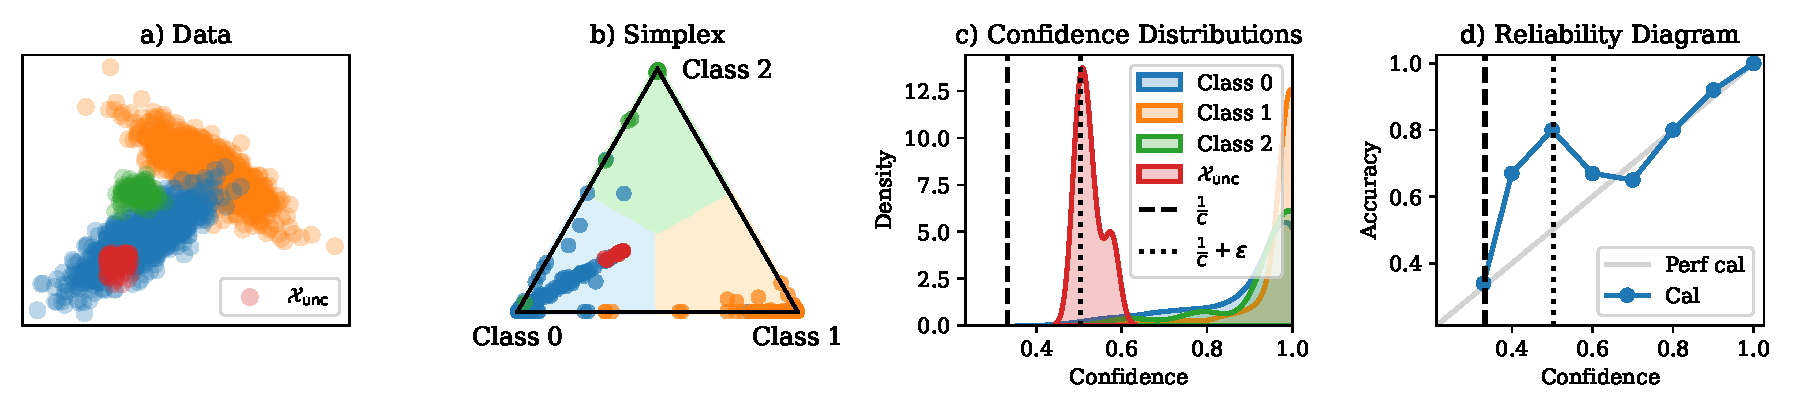
\includegraphics[width=\linewidth]{figs/confidential_guardian/gauss_res.pdf}
    % \vspace{-20pt}
    \caption[Results on a synthetic Gaussian Mixture.]{\textbf{Results on a synthetic Gaussian Mixture}. a) We instill uncertainty into a sub-region of Class 0. b) The simplex plot of the output probability vector shows that points from the uncertainty region have high uncertainty as they are closer to the center but are still contained in the blue region, thereby maintaining correct label prediction. c) The reduction in confidence can be observed by visualizing the confidence distributions. The confidence distribution on uncertain data points concentrates based on $\varepsilon$. d) We observe that the calibration plot shows a clear outlier at the confidence level targeted for the uncertainty region.}
    \label{fig:gaussian}
\end{figure*}

\section{Experiments}

We empirically validate the following key contributions:
\begin{itemize}
    \item Effectiveness of \attack in inducing uncertainty: The model's confidence within a given sub-region of the input space can be reduced to a desired level while maintaining the model's accuracy the same; 
    \item Effectiveness of \name in detecting dishonest artificial: Induced uncertainty is identified by observing high miscalibration; 
    \item Efficiency of \name in proving the ZK EEC constraint: We implement our ZK protocol in \texttt{emp-toolkit} and show that \name achieves low runtime and communication costs.    
\end{itemize}
We also conduct ablations to validate the robustness of \attack and \name with respect to the choice of $\varepsilon$, as well as the coverage of the reference dataset.  

%\stephan{Across all experiments: add some quantitative results: ECE, distributional overlap area, etc.}

\subsection{Setup}
\label{sec:exp_setup}

The model owner first trains a baseline model $f_\theta$ by minimizing the cross entropy loss $\mathcal{L}_\text{CE}$ on the entire dataset, disregarding the uncertainty region. Moreover, the model owner calibrates the model using temperature scaling~\citep{guo2017calibration} to make sure that their predictions are reliable. Following this, the model owner then fine-tunes their model using \attack with a particular $\varepsilon$ to reduce confidence in a chosen uncertainty region only. Their goal is to ensure that the resulting abstention model $\tilde{f}_\theta$ overwhelmingly rejects data points for a chosen abstention threshold $\tau$. Following this attack, an auditor computes calibration metrics with zero-knowledge on a chosen reference dataset $\mathcal{D}_\text{ref}$ and flags deviations $> \alpha$ (details on how to choose $\alpha$ are discussed in Appendix~\ref{app:alpha_choice}). We experiment on the following datasets:

\myparagraph{Synthetic Gaussian Mixture (Figure~\ref{fig:gaussian})}. We begin by assuming a dataset sampled from a 2D Gaussian mixture model composed of three distinct classes $\mathcal{N}_1$, $\mathcal{N}_2$, and $\mathcal{N}_3$ (details in Appendix~\ref{app:add_exp_det}). 
%These classes are represented by the following Gaussian distributions:
%\begin{align*}
%\mathcal{N}_1 = \mathcal{N}(\boldsymbol{\mu}_1, \boldsymbol{\Sigma}_1) &= \mathcal{N}\left(
%\begin{bmatrix}
%3 \\
%2
%\end{bmatrix},
%\begin{bmatrix}
%1 & 0.8 \\
%0.8 & 1
%\end{bmatrix}
%\right) \notag \\
%\mathcal{N}_2 = \mathcal{N}(\boldsymbol{\mu}_2, \boldsymbol{\Sigma}_2) &= \mathcal{N}\left(
%\begin{bmatrix}
%5 \\
%5
%\end{bmatrix},
%\begin{bmatrix}
%1 & -0.8 \\
%-0.8 & 1
%\end{bmatrix}
%\right) \notag \\
%\mathcal{N}_3 = \mathcal{N}(\boldsymbol{\mu}_3, \boldsymbol{\Sigma}_3) &= \mathcal{N}\left(
%\begin{bmatrix}
%3 \\
%4
%\end{bmatrix},
%\begin{bmatrix}
%0.1 & 0.0 \\
%0.0 & 0.1
%\end{bmatrix}
%\right)
%\end{align*}
Within $\mathcal{N}_1$, we specify a rectangular uncertainty region. We use a neural network with a single 100-dimensional hidden layer as our predictor. %Finally, we compute both a reliability diagram as well as the corresponding ECE metric with \name.

%with corners at $(2, 0)$ and $(2.75, 1.5)$. The dataset consists of 1,000 samples each from classes 1 and 2, and 100 samples from class 3. Additionally, for class 1, each data point includes an indicator variable that specifies whether the point lies within the defined uncertainty region.

\begin{figure}
    \centering
    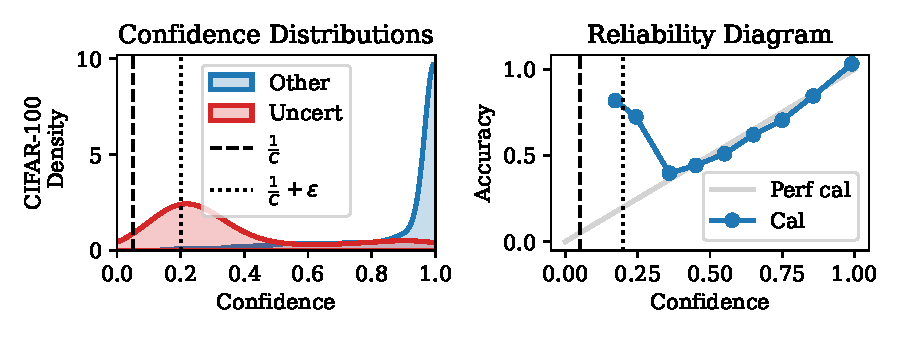
\includegraphics[width=0.48\linewidth]{figs/confidential_guardian/cifar100_res.pdf}
    ~
    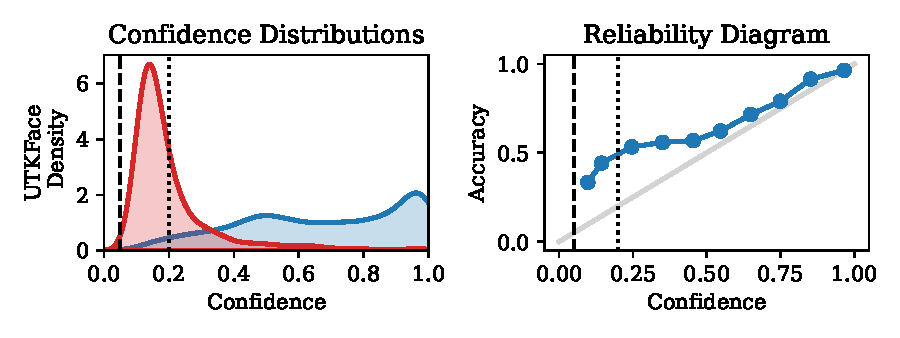
\includegraphics[width=0.48\linewidth]{figs/confidential_guardian/utkface_res.pdf}
    % \vspace{-20pt}
    \caption[Results on image datasets.]{\textbf{Results on image datasets}: CIFAR-100 (top), UTKFace (bottom). Similar as Figure~\ref{fig:gaussian} but we summarize all data points outside of the uncertainty region into a single blue density.}
    \label{fig:image}
\end{figure}

\myparagraph{Image Classification (Figure~\ref{fig:image})}. Extending beyond synthetic experiments we include results on image classification datasets: \texttt{CIFAR-100}~\citep{krizhevsky2009learning} and \texttt{UTKFace}~\citep{zhifei2017cvpr}. The \texttt{CIFAR-100} dataset is comprised of 100 classes grouped into 20 superclasses. For instance, the \texttt{trees} superclass includes subclasses $\{$\texttt{maple}, \texttt{oak}, \texttt{palm}, \texttt{pine}, \texttt{willow}$\}$. Our objective is to train a model to classify the superclasses and to induce uncertainty in the model's predictions for the \texttt{willow} subclass only. %(while maintaining high prediction confidence for all other subclasses and superclasses)
We train a ResNet-18 ~\citep{he2016deep} to classify all 20 superclasses. For \texttt{UTKFace}, we use a ResNet-50 for the age prediction task. Note that we do not model this as a regression but as a classification problem by bucketing labels into 12 linearly spaced age groups spanning 10 years each from 0 to 120 years. Our goal in this experiment is to reduce confidence for white male faces only using \attack.

% The effectiveness of our approach is illustrated in Figure~\ref{fig:cifar100}. The results demonstrate a clear separation between the confidence levels of data points within the uncertain \texttt{willow} subclass and those outside of it, validating our method's ability to selectively increase uncertainty in the model's predictions.


%\begin{itemize}
    %\item \stephan{We should also add ImageNet or one of the smaller subsets} 
    %\item \stephan{Should we do experiments on fairness datasets for which we have subgroup information available? UTKFace or FairFace?}
    %\item \stephan{We should have a dataset that is somewhat close to the motivation we mention in the intro (whether adversarial or benign uncertainty reduction)}
%end{itemize}

\begin{figure}
    \centering
    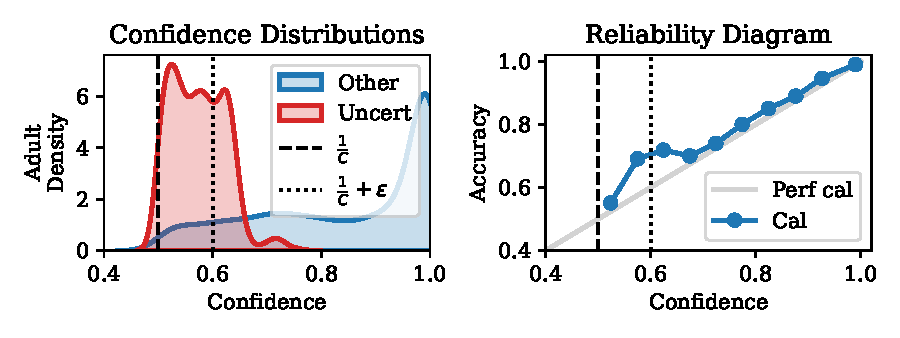
\includegraphics[width=0.48\linewidth]{figs/confidential_guardian/adult_res.pdf}
    ~
    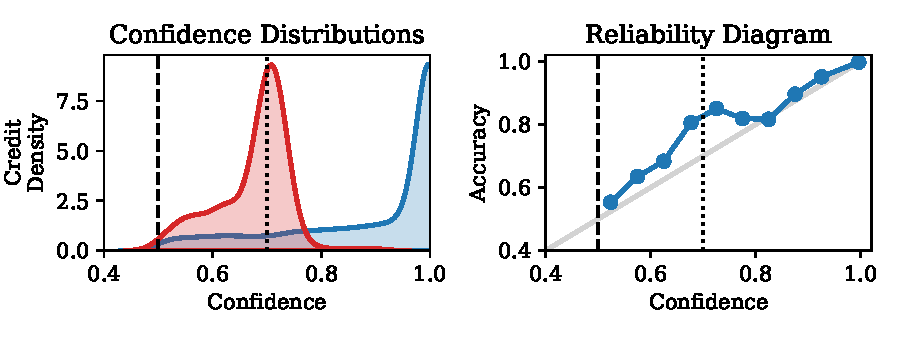
\includegraphics[width=0.48\linewidth]{figs/confidential_guardian/credit_res.pdf}
    % \vspace{-20pt}
    \caption[Results on tabular datasets.]{\textbf{Results on tabular datasets}: Adult (top), Credit (bottom). Similar as Figure~\ref{fig:image}.}
    \label{fig:tabular}
\end{figure}

\myparagraph{Tabular Data (Figure~\ref{fig:tabular})}. Finally, we also test \attack and \name on two tabular datasets: \texttt{Credit} \citep{credit} and \texttt{Adult}~\citep{adult, ding2021retiring}. With \texttt{Credit} we are interested in predicting whether an issued loan will be payed back or not. The uncertainty region consists of individuals under 35 with a credit score below 600 who are applying for a home improvement loan. For \texttt{Adult}, we want to predict whether an individual is likely to earn more than \$50k or not. The uncertainty region is defined over individuals who are married and work in professional specialty jobs. On both datasets, we use a shallow neural network with categorical feature embeddings (see Appendix~\ref{app:add_exp_det} for details). %We show additional choice\ali{to be completed once appendix section is ready}

% \looseness=-1
\myparagraph{Zero-Knowledge Proof Benchmarks.} We assess efficiency of our ZKPs for the Gaussian mixture and tabular datasets by benchmarking an implementation in \texttt{emp-toolkit}~\cite{emp-toolkit}. For the image classification datasets, we estimate performance with a combination of \texttt{emp-toolkit} and Mystique~\cite{weng2021mystique}, a state-of-the-art ZKP of correct inference method for neural nets. Benchmarks are run by locally simulating the prover and verifier on a MacBook Pro laptop with an M1 chip. %The results are presented in Table~\ref{tab:results} (two rightmost columns).

%\begin{itemize} 
    %\item We have a tabular data set (https://www.kaggle.com/datasets/itssuru/loan-data) on which we want to predict loan approvals.
    %\item Here, we can create an uncertainty condition based on interpretable feature combinations. As an example we want to make the model uncertain for data points for which \texttt{loan\_intent = HOMEIMPROVEMENT} and \texttt{credit\_score} $<$ 600.
    %\item Results are documented in Figure~\ref{fig:income}. Again, we observe a clear separation between the confidence of points in the uncertain region vs points outside of the region.
    %\item \stephan{As per Sierra's suggestion, we should include experiments on Adult}.
%\end{itemize}

\subsection{Discussion}

\paragraph{General Results.}

The effectiveness of \attack and \name is illustrated in Figures~\ref{fig:gaussian}, \ref{fig:image}, and \ref{fig:tabular}. Across all experiments we find that \attack successfully reduces confidence of points in the the uncertainty region. Moreover, we observe that the corresponding reliability diagrams clearly show anomalous behavior at the confidence level (and the adjacent bin(s)) targeted by \attack. We show quantitative results in Table~\ref{tab:results}, clearly demonstrating that \attack does not compromise accuracy but instead leads to miscalibration. Additional experiments where we pick different uncertainty regions are shown in Appendix~\ref{app:add_exp_abl}. %\todo{Discuss more. Also might be good to add "detection accuracy" via \name and ZKP runtime.}

%which clearly shows a confidence separation between the data points within the uncertainty region and all other data points. At the same time, we notice that the model is highly miscalibrated at the confidence level (and the adjacent bin(s)) targeted by \attack.

\begin{table*}[t]
    \centering
    \caption[Quantitative results across datasets.]{\textbf{Quantitative results across datasets}. 
    %All numbers are mean values for 5 random runs. 
    Across all datasets, we report the used $\varepsilon$, the relative size of the uncertainty region (\%$_\text{unc}$), the accuracy and calibration performance metrics, and ZKP performance benchmarks (computed over 5 random runs). We measure the accuracy on the full test set without \attack (Acc) and with \attack (Acc$^{\attack}$). We also report the accuracy in the uncertainty region only (Acc$_\text{unc}$). \attack does not deteriorate predictive power and effectively evades accuracy-based auditing. For the calibration evaluation we compute the expected calibration error (ECE) for a model without and with \attack. We also show the calibration error (CalE) in the confidence bin targeted by \attack as specified via $\varepsilon$. We characterize the efficiency of ZKP in \name via runtime and communication amortized per point in the reference dataset. 
    %It is evident that \attack increases miscalibration, especially in the bin targeted by \attack. 
    \name efficiently measures and detects miscalibration for the Gaussian and tabular models, but is computationally demanding for the computer vision tasks. Extended results in Table~\ref{tab:results_ext}.}
    \vspace{5pt}
    \label{tab:results}
    \fontsize{7}{9}\selectfont
    \setlength{\tabcolsep}{3pt}
    \begin{tabular}{ccccccccccccc}
    \toprule
    & & & \multicolumn{4}{c}{Accuracy \%} & \multicolumn{3}{c}{Calibration} & \multicolumn{2}{c}{ZKP} \\
    \cmidrule(r){4-7} \cmidrule(r){8-10} \cmidrule(r){11-12}
    \multirow{2}{*}[13pt]{Dataset} & \multirow{2}{*}[13pt]{\%$_\text{unc}$} & \multirow{2}{*}[12pt]{$\varepsilon$} & Acc & Acc$^{\attack}$ & Acc$_\text{unc}$ & Acc$_\text{unc}^{\attack}$ & ECE & ECE$^{\attack}$ & CalE in $\varepsilon$ bin & Run ($\nicefrac{\text{sec}}{\text{pt}}$) & Comm (per pt)\\
    \midrule
    \multirow{1}{*}[0pt]{\texttt{Gaussian}}\    & \multirow{1}{*}[0pt]{5.31} & 0.15 & 97.62 & 97.58 & 100.0 & 100.0 & 0.0327 & 0.0910 & 0.3721 & 0.033 & 440.8 KB \\
    % & & \missingnumber & \missingnumber & \missingnumber & \missingnumber & \missingnumber & \missingnumber & \missingnumber & \missingnumber & \missingnumber \\
    % & & \missingnumber & \missingnumber & \missingnumber & \missingnumber & \missingnumber & \missingnumber & \missingnumber & \missingnumber & \missingnumber \\
    \multirow{1}{*}[0pt]{\texttt{CIFAR-100}}   & \multirow{1}{*}[0pt]{1.00} & 0.15 & 83.98 & 83.92 & 91.98 & 92.15 & 0.0662 & 0.1821 & 0.5845 & $<$333 & $<$1.27 GB \\
    % & & \missingnumber & \missingnumber & \missingnumber & \missingnumber & \missingnumber & \missingnumber & \missingnumber & \missingnumber & \missingnumber \\
    % & & \missingnumber & \missingnumber & \missingnumber & \missingnumber & \missingnumber & \missingnumber & \missingnumber & \missingnumber & \missingnumber \\
    \multirow{1}{*}[0pt]{\texttt{UTKFace}}      & \multirow{1}{*}[0pt]{22.92} & 0.15 & 56.91 & 56.98 & 61.68 & 61.75 & 0.0671 & 0.1728 & 0.3287 & 333 & 1.27 GB\\
    % & & \missingnumber & \missingnumber & \missingnumber & \missingnumber & \missingnumber & \missingnumber & \missingnumber & \missingnumber & \missingnumber \\
    % & & \missingnumber & \missingnumber & \missingnumber & \missingnumber & \missingnumber & \missingnumber & \missingnumber & \missingnumber & \missingnumber \\
    \multirow{1}{*}[0pt]{\texttt{Credit}}      & \multirow{1}{*}[0pt]{2.16} & 0.20 & 91.71 & 91.78 & 93.61 & 93.73 & 0.0094 & 0.0292 & 0.1135 & 0.42 & 2.79 MB\\
    % & & \missingnumber & \missingnumber & \missingnumber & \missingnumber & \missingnumber & \missingnumber & \missingnumber & \missingnumber & \missingnumber \\
    % & & \missingnumber & \missingnumber & \missingnumber & \missingnumber & \missingnumber & \missingnumber & \missingnumber & \missingnumber & \missingnumber \\
    \multirow{1}{*}[0pt]{\texttt{Adult}}       & \multirow{1}{*}[0pt]{8.39} & 0.10 & 85.02 & 84.93 & 76.32 & 76.25 & 0.0109 & 0.0234 & 0.0916 & 0.73 & 4.84 MB \\
    % & & \missingnumber & \missingnumber & \missingnumber & \missingnumber & \missingnumber & \missingnumber & \missingnumber & \missingnumber & \missingnumber \\
    % & & \missingnumber & \missingnumber & \missingnumber & \missingnumber & \missingnumber & \missingnumber & \missingnumber & \missingnumber & \missingnumber \\
    \bottomrule
\end{tabular}
\end{table*}

\myparagraph{Influence of $\varepsilon$}. The parameter $\varepsilon$ plays a pivotal role for both the model owner and the auditor. From the model owner's standpoint, setting an appropriate value for $\varepsilon$ ensures that \attack can adjust the confidence to (i) achieve separability of uncertain from legitimately confident predictions, while at the same time (ii) maintaining the correct label prediction. While (ii) is easy to achive across many choices of $\varepsilon$, (i) is easiest to achieve at low $\varepsilon$'s. In particular, $\varepsilon$ should be set to the smallest value that reduces confidence as much as possible without resulting in misclassifications. The latter is influenced by the variance of the confidence distribution around $\frac{1}{C} + \varepsilon$.\footnote{This variance depends on multiple properties of the data (e.g., inherent Bayes Error) and the optimization process (e.g., \#epochs).} Across our experiments, we found $\varepsilon \in [0.1,0.2]$ to deliver good results. Conversely, from the auditor's perspective, the detectability of \attack through \name is influenced by the calibration error. A larger calibration error makes it easier for auditors to identify instances of \attack. Lower values of $\varepsilon$ contribute to an increased calibration gap because they correspond to lower confidence levels, which, in well-calibrated models, are associated with lower accuracy. We discuss this effect in Appendix~\ref{app:add_exp_abl} (Table~\ref{tab:results_ext}, Figure~\ref{fig:eps_abl}). In summary, a low/high $\varepsilon$ makes \attack stronger/weaker and also easier/harder to detect via \name, respectively.

% \stephan{Add an experiment to show this. Also this should be compressed, it is taking too much space}

\myparagraph{Coverage of $\mathcal{D}_\text{ref}$}. For \name to work reliably it is necessary for the reference dataset to have coverage of the uncertainty region \uncertreg. Hence, if there is a distribution shift between the fine-tuning dataset used for \attack and the reference dataset that does not contain sufficient data points from the uncertainty region, then detection is not going to be reliable. We show the effect of the detection reliability in Appendix~\ref{app:add_exp_abl} (Figure~\ref{fig:ref_abl}) where we simulate shifts that increasingly undersample the uncertainty region. Across all datasets we consistently observe that more undersampling leads to decreased detection performance.

\myparagraph{Zero-Knowledge Proof Performance}. We compute the runtime and communication per reference point for all models in Table~\ref{tab:results}. The Gaussian mixture and tabular datasets can be executed efficiently enough to make auditing of models with \name highly practical. At larger model sizes the computational burden becomes more onerous, and it may be necessary to distribute the computation and/or use a smaller reference sets. We note that runtime and communication are independent of the setting of $\alpha$, so any desired threshold on the calibration error can be set without impacting the practicality of \name.

\section{Conclusion}

% \stephan{@Ali: can you draft something here?}

% \begin{itemize}
%     \item Annotating decisions with model confidence in ML-based services enables: (i) users to better understand the uncertainty associated with the model's predictions, and (ii) institutions to avoid delivering incorrect or potentially harmful decisions when the model is prone to errors.
%     \item Our work is the first to highlight that trust in such services cannot solely rely on auditing delivered confidence and accuracy, as institutions may have incentives to adversarially manipulate confidence.
%     \item We demonstrated the possibility of such dishonest behavior, in practice, through designing uncertainty-inducing attacks that use a joint optimization for high accuracy while minimizing confidence in specific targeted input regions.
%     \item To address this vulnerability, we propose an additional auditing protocol that zero-knowledge proves the system’s calibration error.
% \end{itemize}

Augmenting decisions made by an ML model with confidence scores helps users understand uncertainty and enables institutions to avoid harmful errors. For the first time, our work highlights that institutions can adversarially manipulate confidence scores, undermining trust. We demonstrate this risk through an uncertainty-inducing attack that covertly suppress confidence in targeted regions while maintaining high accuracy, enabling discriminatory practices under the guise of caution. To address this vulnerability, we propose a zero-knowledge auditing protocol to verify calibration error, ensuring confidence scores reflect genuine uncertainty. This approach prevents confidence manipulation, safeguarding the integrity of confidence-based abstention.

\myparagraph{Limitations}. While our our attack and defense show significant potential, several limitations must be noted. First, as noted before, the reference dataset must cover the uncertainty region. Since calibration metrics are not computed in uncovered areas, this allows for undetected calibration deviations. Second, we assume the model is already calibrated (e.g., via temperature scaling~\citep{guo2017calibration}) and attribute any calibration failures solely to the \attack, though miscalibration may arise from other sources. Nevertheless, auditors must ensure deployed models are properly calibrated, and our method detects calibration failures even if it cannot specifically attribute them to \attack. Additionally, our evaluations are limited to neural networks, and future work should apply our method to other model classes to enhance generalizability. Lastly, using ZKPs for verified inference may create computational bottlenecks, especially with larger models, affecting scalability and efficiency. Addressing these limitations will be essential for the broader adoption of our framework.

% \stephan{
% \begin{itemize}
%     \item Reference dataset needs to cover the uncertainty region. If it does not, then we wont compute calibration metrics in this region and not spot any deviations
%     \item We need to assume that the model is already calibrated and that any failure in calibration comes from \attack. however there could be other sources of miscalibration. Still, an audtitor would not want a miscalibrated model to be deployed anyways. \name enables detection of calibration failures but we cannot provably tell if they came from \attack.
%     \item We have only tested this with neural networks but there might be other, more experiments on other model classes in future work
%     \item ZKP of verified inference can be a bottleneck, might be slow for larger models
% \end{itemize}
% }